\documentclass[a4paper]{article}
%\usepackage[top=30pt,left=30pt,right=30pt]{geometry}
\usepackage[german,english]{babel}
%\usepackage[utf8]{inputenc}
\usepackage{amsmath}
\usepackage{amssymb}
\usepackage{amsthm}
\usepackage{graphicx}
\usepackage{caption}
\usepackage{fontspec}
\usepackage{mdframed}
\usepackage{pxfonts}
\usepackage{wasysym}
\usepackage{framed}
\usepackage{xcolor}
\usepackage{makeidx}
\usepackage{csquotes}
\usepackage[pdfborder={0 0 0}]{hyperref}
\usepackage{stmaryrd}
\usepackage{titlesec}
\titleformat{\paragraph}{\normalfont\itshape}{}{}{}

\newcounter{lecref}[section]
\numberwithin{lecref}{section}
\setcounter{section}{-1}
\newcounter{exercises}

\newtheorem{theorem}[lecref]{Theorem}
\newtheorem*{Theorem}{Theorem}
\newtheorem{example}[exercises]{Example}
\newtheorem*{Example}{Example}
\newtheorem{definition}[lecref]{Definition}
\newtheorem*{Definition}{Definition}
\newtheorem{lemma}[lecref]{Lemma}
\newtheorem*{Lemma}{Lemma}
\newtheorem{claim}[lecref]{Claim}
\newtheorem*{Claim}{Claim}
\newtheorem{remark}[lecref]{Remark}
\newtheorem*{Remark}{Remark}
\newtheorem{algorithm}[lecref]{Algorithm}
\newtheorem*{Algorithm}{Algorithm}
\newtheorem{corollary}[lecref]{Corollary}
\newtheorem*{Corollary}{Corollary}
\newtheorem{proposition}[lecref]{Proposition}
\newtheorem*{Proposition}{Proposition}
\newtheorem{revision}{Revision}
\newtheorem*{Revision}{Revision}

\def\ifempty#1{\def\temp{#1} \ifx\temp\empty }

% useful control sequences for mathematical notation
\newcommand{\Abs}[1]{\left|#1\right|}
\newcommand{\Set}[1]{\left\{#1\right\}}
\newcommand{\SetDef}[2]{\left\{#1\,\mid\,#2\right\}}
\newcommand{\IP}[2]{\left\langle#1, #2\right\rangle}
\newcommand{\Norm}[1]{\left\|{\ifempty{#1}\cdot\else#1\fi}\right\|}
\newcommand{\Max}[1]{\max{\Set{#1}}}
\newcommand{\Min}[1]{\min{\Set{#1}}}
\newcommand{\Sup}[1]{\sup{\Set{#1}}}
\newcommand{\Powerset}[1]{{\mathbb P}(#1)}
\newcommand{\IntRange}[2]{#1, \dots\ifempty{#2}\else, #2\fi}

\def\vec2#1#2{\begin{pmatrix} #1 \\ #2 \end{pmatrix}}
\def\vec3#1#2#3{\begin{pmatrix} #1 \\ #2 \\ #3 \end{pmatrix}}
\newcommand{\noproof}[1]{A proof for Theorem~\ref{#1} is not provided.}
\newcommand{\dotted}[1]{\:\dot{#1}\:}  % dot has too little margin

% German translation
\newcommand{\dt}[1]{(dt. \enquote{\foreignlanguage{german}{#1}})}

% essential control sequences
%% \xRightarrow: \xrightarrow for \rightarrow like \xRightarrow for \Rightarrow
\makeatletter
\newcommand{\xRightarrow}[2][]{\ext@arrow 0359\Rightarrowfill@{#1}{#2}}
\makeatother

% typesetting settings
\parindent0pt
\setlength{\parskip}{.6em}
\setmainfont{CMU Serif Roman}

% TODO: span?
\DeclareMathOperator{\rank}{rank}
\DeclareMathOperator{\diag}{diag}
\DeclareMathOperator{\detm}{det}
\DeclareMathOperator{\perm}{perm}
\DeclareMathOperator{\sign}{sign}
\DeclareMathOperator{\degree}{deg}
\DeclareMathOperator{\im}{image}
\DeclareMathOperator{\ke}{kernel}
\DeclareMathOperator{\spec}{spec}
\DeclareMathOperator{\prop}{probability}
\DeclareMathOperator{\Hom}{Hom}
\DeclareMathOperator{\argmax}{argmax}
\DeclareMathOperator{\argmin}{argmin}
\DeclareMathOperator{\vol}{vol}  % volume
\DeclareMathOperator*{\bigtimes}{\vartimes}





\newcommand{\dateref}[1]{%
  \begin{mdframed}[backgroundcolor=gray!10,innerbottommargin=0pt,innertopmargin=0pt]
    \paragraph{\textit{$\downarrow$ This lecture took place on #1.}}%
  \end{mdframed}%
}

% metadata
\title{
  Optimization 1 \\
  \large{Lecture notes, University of Technology, Graz} \\
  based on the lecture by Bettina Klinz
}
\date{\today}
\author{Lukas Prokop}

\makeindex
\begin{document}

\maketitle
\tableofcontents

\section{Course}

\dateref{2019/03/04}

\begin{itemize}
	\item Lecture
	\begin{itemize}
		\item Monday, 12:15--14:00
		\item Tuesday, 16:15--18:00
	\end{itemize}
	\item First week, the practicals session will be used for the lecture
	\item Practicals will take place usually on Wednesday, 16:15--18:00 \\
		in exceptional cases on Thursday, 16:15--18:00
	\item 2 websites (work in progress):
		\begin{itemize}
			\item \url{http://www.math.tugraz.at/~klinz/optimvo} (list of literature)
			\item \url{http://www.math.tugraz.at/~klinz/optimue} (practicals mode, practicals exercises, additional content)
		\end{itemize}
	\item Two large topics in this lecture
		\begin{itemize}
			\item Linear optimization (linear target function, linear side conditions)
			\item Non-linear optimization without sub conditions (unconstrained non-linear optimization) \\
				where non-linear optimization denotes that the target function is non-linear
		\end{itemize}
	\item Be aware, that this class might be the lecture requiring previous results of classes the most.
	\item Advanced lecture in masters
		\begin{itemize}
			\item Lecture \enquote{Non-linear optimization} (includes nonlinear optimization with sub conditions)
		\end{itemize}
	\item Exam
		\begin{itemize}
			\item written + orally, in case of negotiation and few candidates only orally
			\item 1st date will be at the end of the semester, optionally in summer holidays
			\item 2 written exams for the practicals
		\end{itemize}
\end{itemize}

\subsection{Linear optimization}

We have already seen optimization problems in high school or previous semesters.
But, for example, handling constraints consisting of inequalities was tedious or trivial.
We consider more sophisticated techiques here.
In practice, linear models occur rarely. But they often provide a sufficient heuristic.

\subsection{Introduction and some examples for linear optimization models}

\begin{example}[Production planning model]
	\label{example:1}
	A factory can produce $n$ goods.
	The revenue per unit of good $j$ is given by $c_j$ units of money.
	Production is limited by restrictions, that result from constrained availability of staff, equipment and raw materials.
	Let $m$ denote the number of these resources and $b_i$ is the maximum availability of resource $i$ ($i = 1, \dots, m$).
	Let $a_{ij}$ with $1 \leq i \leq m$ and $1 \leq j \leq n$ denote the quantity of resource $i$ required to produce 1 unit of good $j$.
	Our goal is to maximize revenue with respect to the given constraints.

	\emph{Decision variable:} $X_j$ is the quantity of good $j$

	\[ \text{target function: } \max \sum_{j=1}^n c_j x_j \]
	\[ \text{ subject to (constraints) } \sum_{j=1}^n a_{ij} x_j \leq b_i \qquad i \in \Set{1, \dots, m} \]
	\[ \text{ with } x_j \geq 0 \qquad \text{ sign condition} \]

	Pay attention! We do not require $x_j \in \mathbb Z$. For $x_j \in \mathbb Z$ we get an integral linear program which is \emph{not} a linear programm! (this is a difficult subproblem of optimization)
\end{example}

\begin{example}[Mixture problem]
	\label{example:2}
	Consider $n$ kinds of raw materials. Our goal: We want to create a new material by mixing existing raw materials to reduce costs.

	\begin{Example}[Alloys]
		Consider $n$ different base alloys $L_1, \dots, L_n$.
		For each material we have the lead content in percent ($a_1, \dots, a_n$) and the costs per unit of weight ($c_1, \dots, c_n)$.
		We have to produce alloys with lead content $b \%$.
		The decision variable $x_j$ is given by the ratio of $L_j$.

		Formally, the problem can be defined as
		\[ \min{\sum_{j=1}^n c_j x_j} \text{ s.t. } \sum_{j=1}^n x_j = 1, \sum_{j=1}^n a_j x_j = b, x_j \geq 0 \]
		These are typical mixture constraints and they ensure a given lead content.
	\end{Example}
\end{example}

\begin{example}[Linear transportation problem]
  \label{example:3}
  Given $m$ firms, $n$ customers, $a_i$ is the offer by firm $i$ and $b_j$ is the demand by customer $j$.
  $c_{ij}$ are the transportation costs from firm $i$ to customer $j$.

  Find an admissible transportation plan with minimal costs.
  The decision variable $x_{ij}$ is the quantity of goods transported from firm $i$ to customer $j$.

  Formally,
  \[ \min{\sum_{i=1}^m \sum_{j=1}^n c_{ij} x_{ij}} \text{ s.t. } \sum_{i=1}^m x_{ij} = b_j, \sum_{j=1}^n x_{ij} = a_i, x_{ij} \geq 0 \quad j \in \Set{1, \dots, n}, i \in \Set{1, \dots, m} \]
\end{example}

\begin{Example}[Diet problem]
  The following problem has a strong historical background in optimization sciences:
  Stigler diet problem (in the year 1939) by Georg Stigler. 

  Given a list of 77 ingredients. Per ingredient we are given features such as calories and proteins.
  Find an optimal combination to minimize costs.

  His heuristic results were confirmed as almost optimal in 1947.
\end{Example}

In the following lectures, our goal will be:

\begin{itemize}
	\item Theory of linear optimization (Knowledge about fundamentals and background)
	\item Algorithmic solutions procedures: in the lecture we will discuss two procedures:
		\begin{itemize}
			\item Simplex process (G. Dantzig, 1947, in practice useful, no polynomial runtime)
			\item Inner point method (in practice useful, polynomial runtime)
		\end{itemize}
		Outside this lecture:
		\begin{itemize}
			\item Ellipsoid method: polynomial runtime, but in practice useless
		\end{itemize}
\end{itemize}

\section{Geometrical considerations of linear optimization}

\begin{Definition}
  Standard form of a linear program (canonical representation)
  \[ \max{z(x)} = z_0 + \sum_{j=1}^n c_j x_j \text{ such that } \sum_{j=1}^n a_{ij} x_j \leq b_i, x_j \geq 0 \qquad i \in \Set{1, \dots, m} \]
  In compact notation:
  \[ \max{z_0 + c^t x} \text{ s.t. } Ax \leq b, x \geq 0 \]
  typically $\max c^t x$.
  $z_0$ does not influence the result.

  \[ A = \begin{pmatrix} a_{11} & \dots & a_{1n} \\ \vdots & \ddots & \vdots \\ a_{m1} & \dots & a_{mn} \end{pmatrix} \qquad b = \begin{pmatrix} b_1 \\ \vdots \\ b_m \end{pmatrix} \qquad a_{ij} \in \mathbb R, b_i \in \mathbb R, c_j \in \mathbb R \]
\end{Definition}

\dateref{2019/03/05}

\begin{Revision}
	The canonical/standard form of a linear program is given by
	\[ \max c^t x \text{(} + \text{optionally } z_0 \text{) such that } Ax \leq b \qquad x \geq 0 \]
\end{Revision}

\begin{Remark}[Observation]
  Every arbitrary linear program (min/max of an affine linear function over a linear constraint) can be transformed into the canonical form above.
  \begin{enumerate}
  	\item The minimization over $c^t x$ corresponds to $-c^t x$ as maximization problem.
  	\item Constraints of form $\alpha^t x \geq b$ can be written as $-\alpha^t x \leq -\beta$.
  	\item A constraint of form $\alpha^t x = \beta$ can be written as $\alpha^t x \leq \beta$ with $\alpha^t x \geq \beta$. Or equivalently as $\alpha^t x \leq \beta$ with $-\alpha^t x \leq -\beta$.
  		\begin{Remark} \hfill
	  		\begin{itemize}
	  			\item Disadvantage: One constraint is transformed into two.
	  			\item In practice, the explicit handling of equality constraints should be preferred.
	  		\end{itemize}
  		\end{Remark}
  	\item Let $x_j$ not be restricted w.r.t. the sign. Write $x_j$ as $x_j = x_j^+ - x_j^-$ with $x_j^+ \geq 0$ and $x_j^- \geq 0$.
  		$x_j$ will be replaced by $x_j^+ - x_j^-$ with $x_j^+ \geq 0$ and $x_j^- \geq 0$.
  		\begin{Remark}
  			Disadvantage: Number of variables is increased.
  		\end{Remark}
  \end{enumerate}
\end{Remark}

\begin{Remark}[Terminology] \hfill{}
  \begin{itemize}
  	\item 2 points $u, v \in \mathbb R^n$ define a \emph{line} $G(u, v) = \SetDef{u + \lambda (v - u)}{\lambda \in \mathbb R}$. \index{Line}
  	\item A \emph{halfline} is formally given by $\SetDef{u + \lambda (v - u)}{\lambda \geq 0}$ \index{Halfplane}
  	\item A \emph{closed interval} (or \emph{segment}) is defined as $[u, v] = \SetDef{u + \lambda (v - u)}{\lambda \in [0, 1]}$ and
  		an \emph{open interval} is defined as $(u, v) = \SetDef{u + \lambda (v - u)}{\lambda \in (0, 1)}$. \index{Segment}\index{Open interval}\index{Closed interval}
  \end{itemize}
\end{Remark}

\begin{lemma}
	\label{lemma:1.1}
	\begin{itemize}
		\item An affine linear function $z_0 + c^t x$ takes up its maximum/minimum in segment $[u, v]$ in its end points $u$ or $v$.
		\item An affine linear function $z_0 + c^t x$ takes up its maximum/minimum on a half-line in the end points.
	\end{itemize}
\end{lemma}
\begin{proof}
	Left as an exercise to the reader (use parameter representation and insert it into the function)
\end{proof}

\subsection{Hyperplane and Halfspaces}

By the linear inequality $\alpha^t x \leq \beta$ ($\alpha \in \mathbb R^n, \beta \in \mathbb R$) with $\alpha \neq 0$ (zero vector) we define a \emph{closed halfspace}\index{Closed halfspace}.
\[ H_{\leq} \coloneqq \SetDef{x \in \mathbb R^n}{\alpha^t x \leq \beta} \]
Analogously we can define open halfspaces\index{Open halfspace}:
\[ H_{<} \coloneqq \SetDef{x \in \mathbb R^n}{\alpha^t x < \beta} \]
Hyperplane\index{Hyperplane}:
\[ H_{=} \coloneqq \SetDef{x \in \mathbb R^n}{\alpha^t x = \beta} \]
In $\mathbb R^2$, hyperplanes are halflines.
In $\mathbb R^3$, hyperplanes are halfplanes.

\begin{figure}[t]
	\begin{center}
		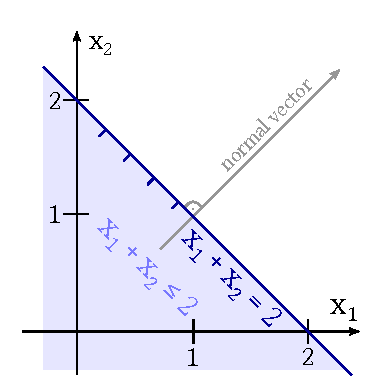
\includegraphics{img/02_constraint.pdf}
		\caption{Constraint $x_1 + x_2 \leq 2$ visualized in $\mathbb R^2$. To determine the halfplane (bright blue) resulting from the constraint, it helps to express the constraint with $x_2$ on the left-hand side: $x_2 \leq 2 - x_1$. Then determine $x_2$ for two different $x_1$ assuming an equality operator, e.g. $x_1 = 0$ with $x_2 = 2$ and $x_1 = 1$ with $x_2 = 1$. Then choose some large value $x_1$ and $x_2$ (e.g. $x_1 = 10$ and $x_2 = 10$). Does it satisfy $x_1 + x_2 \leq 2$? No, the halfplane containing $(10, 10)$ is not the one, we are looking for. Some people prefer to consider the normal vector. Sometimes dashes are used to mark the side of the considered halfplane.}
		\label{img:constraint-vis}
	\end{center}
\end{figure}

Possible cases for the position of lines $G(u, v)$ w.r.t. to the hyperplane $H = \SetDef{x}{\alpha^t x = \beta}$.
\begin{description}
	\item[Case 1] Line $G$ is contained in $H$ (denoted $G \subseteq H$) \\
		$\alpha^t u = \beta$, $\alpha^t (u - v) = 0$
	\item[Case 2] $G$ is parallel to $H$ \\
		$\alpha^t u \neq \beta$, $\alpha^t (u - v) = 0$
	\item[Case 3] $G$ intersects $H$ in one point $c$ \\
		$\alpha^t(u - v) \neq 0$
\end{description}

\begin{lemma}
  \label{lemma:1.2}
  If the line $G(u, v)$ is neither contained in halfplane $H = \SetDef{x}{\alpha^t x = \beta}$ nor in some open halfspace constrained by $H$, $G$ intersects the halfplane $H$ in one point.
\end{lemma}

\begin{Remark}[Observation]
  The parameter representation of a line is ambiguous. We can choose $u$ und $v$ wisely: $G(u, v), \overline{x} \in G$.
  We can always choose $u$ and $v$ such that $\overline{x} \in (u, v)$.

  Let $\overline{x} \in H_{<} = \SetDef{x \in \mathbb R^n}{\alpha^t x < \beta}$. If $G \subseteq H_<$, then $u, v \in H_<$.
  Otherwise, due to $\overline{x} \in G \cap H_{<}$, $G$ intersects the hyperplane $H = \SetDef{x \in \mathbb R^n}{\alpha^t x = \beta}$.

  Furthermore we can choose a representation $(u, v)$ such that $\overline{x} \in (u, v) \subseteq H_{<}$ and $v \in H_{=}$.
  This can be generalized to multiple halfspaces.
\end{Remark}

\begin{Definition}
  A \emph{polyhedron}\index{Polyhedron}\dt{Polyeder} is the intersection of finitely many halfspaces.
  A bounded polyhedron is also called \emph{polytope}\index{Polytope}.

  % TODO Boundaries of a polyhedron in $\mathbb R^2$, A polytope in $\mathbb R^2$ 
\end{Definition}

\begin{Remark}[Observation]
  The admissible set $P(A, b)$ of the linear program (given in the previous revision) is a polyhedron.
\end{Remark}

\begin{lemma}
  \label{lemma:1.3}
  Halfspaces and thus also polyhedrons are convex sets.
\end{lemma}

Furthermore affine-linear functions are convex \emph{and} concave.
Linear optimization is a special case of convex optimization minimizing a convex function over a convex set.
The neat property of such convex optimization tasks is that local and global minima/maxima collapse (just like in the linear case).

\paragraph{Geometric illustration for $n=2$}
$n=2$ means that we consider $2$ variables.
\[ \max c_1 x_1 + c_2 x_2 \qquad a_{i1} x_1 + a_{i2} x_2 \leq b_i \quad i = 1, \dots, m \qquad x_1, x_2 \geq 0 \]

\begin{figure}[t]
	\begin{center}
		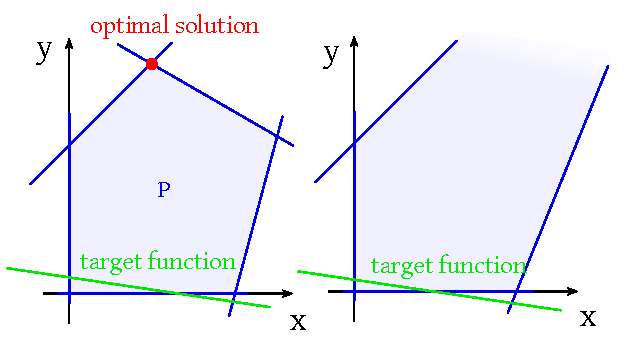
\includegraphics{img/01-bounded-set.pdf}
		\caption{Bounded (left) and unbounded (right) sets. The unbounded set does not have an optimal solution.}
		\label{img:boundedness}
	\end{center}
\end{figure}

\begin{Remark}[Observation]
  Optimal solutions occur at vertices of the set (intersection of two constraints). Compare with Figure~\ref{img:boundedness}.
\end{Remark}

This approach provides a graphical solution method for linear programs with 2 variables.

The generic geometric consideration of a polyhedron is
\[ P = \SetDef{x \in \mathbb R^n}{Ax \leq b} \qquad A \in \mathbb R^{m \times n} \]
Without loss of generality, we assume all row vectors $a_i$ of $A$ are non-zero.
\[ H_i \coloneqq \SetDef{x \in \mathbb R^n}{a_i^t x = b_i} \qquad \text{$i$-th halfplane} \quad i = 1, \dots, m \]

Let $I \subseteq \Set{1, \dots, m}$. Consider
\[ \hat H_I \coloneqq \bigcap_{i \in I} H_i = \SetDef{x \in \mathbb R^n}{a_i^t x = b_i \text{ for } i \in I} \qquad \text{ affine subspace of } \mathbb R^n \]
If $\hat H_I \cap P \neq P \neq \emptyset$, then this set is called \emph{face}\index{Face} of $P$.
The face of $P$ is called minimal\index{Minimal face}, if it does not contain any other face properly.

\begin{Example}
	A cube in $\mathbb R^3$ has 27 faces:
	\begin{itemize}
		\item The cube itself, $I = \emptyset$
		\item 6 faces, $I = \Set{1}, I = \Set{2}, \dots, I = \Set{6}$
		\item 12 face edges, $\Abs{I} = 2$
		\item 8 vertices, $\Abs{I} = 3$
	\end{itemize}
\end{Example}

\begin{Example}[Faces in the left subfigure in Figure~\ref{img:boundedness}]
	11 faces in total (5 vertices of dimension 0, 5 with dimension 1, 1 with dimension 2)
\end{Example}

More formally:
Let $P$ be described by a hyperplane $H_i$ ($a_i^t x = b_i$).
Let $S \subseteq \mathbb R^n, S \neq 0$.
\begin{Definition}
	$I(S) \coloneqq \SetDef{i \in \Set{1, \dots, m}}{S \subseteq H_i}$
\end{Definition}
For $S = \Set{x_0}$, we write $I(x_0)$ instead of $I(\Set{x_0})$.

\begin{Definition}
	\[ L(S) \coloneqq \SetDef{x}{a_i^t x = b_i, i \in I(S)} \]
	is the smallest affine subspace containing $S$.
	For a non-empty $S$, $S$ is a face iff $S = L(S) \cap P$.

	If $S$ is a minimal face, then $S = L(S)$ ($L(S)$ is then a part of the polyhedron).
\end{Definition}

\begin{Definition}[Dimension of a face]
	\[ \dim{S} \coloneqq \dim{L(S)} \]
	so the dimension of the smallest affine subspace containing $S$.
\end{Definition}
\begin{Definition}[Vertex]
	A vertex is a face of dimension $0$.
\end{Definition}
\begin{Remark}
	For polyhedron, the vertex term from above is an alternative definition for the vertex term for convex sets (the terms correspond).
\end{Remark}
\begin{Remark}
	A circle has infinitely many vertices; not none.
\end{Remark}

Let $S$ be convex set in $\mathbb R^n$.
$x$ is called vertex of $S$ if it is not possible to represent $x$ as $x = y + (1 - \lambda) z$ with $y, z \in S, y \neq z, \lambda \in [0,1]$.

\dateref{2019/03/06}

% TODO Problem with two parallel boundaries.

Not every polyhedron has vertices. For example, if the boundaries are given as two parallels, then no vertices can be identified.

\begin{Remark}
	The problem with two parallels is not representable in canonical form.
\end{Remark}

\begin{Definition}
	\index{Acute polyhedron}
	A polyhedron \emph{with} vertices is called \emph{acute}.
\end{Definition}

A vertex is a minimal face.
A face results as unique solution of the corresponding equation system.
\[ a_i^t x = b_i \qquad \forall i \in I(z) \]
If face $S = L(\overline{x}) \cap P$ for $\overline{x} \in \overline{P(A, b)} \eqqcolon P$ has dimension $\geq 1$ (hence no vertex),
then you can let some line $G$ pass through $\overline{x}$ that lies in $L(\overline{x})$.

$\overline{x}$ lies in the intersection of open halfspaces $\SetDef{x}{a_i^t x < b_i, i \not\in I(\overline{x})}$.
Thus we can provide a representation of line $G$ passing through two points $c$ and $d$ with $c, d \in S, \overline{x} \in (c, d)$.

Assume the halfspace with end point $\overline{x}$ in direction $d$ is bounded by some of the constraining hyperplanes of these open halfspaces.
Then $d$ can be chosen as the closest intersection point of the line with one of these hyperplanes $H_i$ for $i \not\in I(\overline{x})$.
\[ \implies \Abs{I(d)} > \Abs{I(\overline{x})} \qquad \implies \dim{L(d)} < \dim{L(\overline{x})} \]

Analogously, the same applies to the constraint by the halfline with end point $\overline{x}$ and in direction $c$.
$\dim{L(c)} < \dim{L(\overline{x})}$. Step by step, we can reduce the dimension to end up with a vertex.

\begin{theorem}[Statement about acute-angled polyhedrons]
	\label{theorem:1.4}
	\begin{enumerate}
		\item A non-empty polyhedron is acute iff it does not contain any line.
		\item Every face of an acute polyhedron contains one vertex.
		\item A polyhedron has (at most) finitely many vertices.
	\end{enumerate}
\end{theorem}
\begin{proof}
	\begin{enumerate}
		\item[1a.]
			Assume $P$ does not contain any lines. Let $x_0 \in P$ ($P \neq 0$).
			If $x_0$ is a vertex, then $P$ is acute. If $x_0$ is not a vertex, then consider the face $S \coloneqq L(x_0) \cap P$.
			Then $\dim{S} \geq 1$ holds true. Now we use the idea, that was sketched above right before the theorem.

			We choose a line $G(c, d) \subseteq L(x_0)$ where $c$ and $d$ are chosen as described before.
			Because $P$ does not contain a line, $S$ also does not contain any.
			Without loss of generality, we assume that the halfline with end point $x_0$ in direction $d$ is bounded and thus $\dim{L(d)} < \dim{L(x_0)}$.
			If $d$ is not a vertex, repeat this construction with some new $x_0 = d$.

			In every step, we are losing at least one dimension. After at most $n$ steps, we are going to have a vertex.
		\item[1b.]
			Let $P$ be acute, then $P$ has a vertex.
			Choose a vertex $\overline{x}$ and $n$ inequalities with maximum row rank.
			$I \subseteq I(\overline{x})$, submatrix $A_I$ of $A$ has $\rank(A_I) = n$.

			Assume there exists a line $G(u, v)$ with $u \neq v$, that in entirely contained in $P$.
			The inequalities $A_I u + \lambda \cdot A_I (v - u) \leq b_I$ must be true for all $\lambda \in \mathbb R$.

			Because $\lambda$ is unbounded, it should be true that $A_I(v - u) = 0$ where $A_I$ is a matrix of full rank.
			So $v - u = 0 \implies v = u$. This is a contradiction.
		\item[2.]
			A face $S$ of an acute polyhedron $P$ cannot contain any line because $S \subseteq P$ und $S$ is itself a polyhedron.
			By the first statement, $S$ has one vertex.
		\item[3.]
			Let $P$ be described by some $m \times n$ matrix $A$.
			$\Set{1, \dots, m}$ has only finitely many subsets.
			Thus we have only finitely many faces.
			\[ \leq {m \choose n} \text{ vertices} \]
	\end{enumerate}
\end{proof}

\begin{Remark}
  By Theorem~\ref{theorem:1.4}, it is immediate that non-empty polyhedrons, that result from linear programs in canonical form,
  $P = \SetDef{x \in \mathbb R^n}{Ax \leq b, x \geq 0}$ are always acute. So it has at least one vertex
  (because the set $\SetDef{x \in \mathbb R^n}{x_i \geq 0, i \in \Set{1, \dots, n}}$ does not contain a line).
\end{Remark}

\subsubsection{Fundamental theorem of Linear Optimization}

\begin{theorem}[Fundamental theorem of Linear Optimization]
  \label{theorem:1.5}
  \begin{enumerate}
  	\item
	  If an affine-linear function $z(x)$ takes up its maximum/minimum in a polyhedron $P$ in $\overline{x} \in P$, then also in all points of face $S = L(\overline{x}) \cap P$.
	\item
	  Especially the optimum is taken up in a vertex of $P$, if $P$ is acute.
  \end{enumerate}
\end{theorem}

\begin{proof}
	\begin{enumerate}
	\item
	  Let $\overline{x}$ be a maximum (analogously for minima) and let $y \neq \overline{x}$ be another point at $S$.
	  Then the line $G \coloneqq G(\overline{x}, y)$ in $L(\overline{x})$.
	  For $G$ there exists a representation $G = G(c, d)$ with $c, d \in P, \overline{x} \in (c, d)$.
	  By Lemma~\ref{lemma:1.1} the affine-linear function $z(x)$ takes up its maximum in line segment $[c, d]$ in $c$ or $d$.
	  Without loss of generality, we assume its maximum in $c$.
	  Thus $z(c) \geq z(\overline{x})$, because $\overline{x} \in (c, d)$.

	  On the other hand, we have $z(\overline{x}) \geq z(c)$, because $c \in P$ and the maximum is reached in $\overline{x}$.

	  Thus $z(c) = z(\overline{x})$. Hence, $z(x)$ is constant in $G$ and therefore $z(y) = z(\overline{x})$.
	  $y$ was chosen arbitrarily, then $z$ is constant at face $S$.
	\item
	  Follows by Theorem~\ref{theorem:1.4} (b).
	\end{enumerate}
\end{proof}

The polyhedron for linear programs in canonical form are empty or acute (have vertices).
The Fundamental theorem of Linear Optimization followingly states that for such linear programs (and thus any linear program becausc every linear program can be represented in canonical form) it suffices to investigate all vertices.

\begin{corollary}
	\label{corollary:1.6}
	If $\max\Set{c^\bot x: x \in P}$ has a linear optimization solution $x^*$, then $c^t x^* = \max\Set{c^t x: x \in V(P)}$ where $V(P)$ is the set of vertices of $P$.
\end{corollary}

Thus we retrieve a finite method for linear programs:
Determine all vertices and filter the vertex optimizing the target function.

\begin{Remark}[Disadvantage]
	Because there are exponentially (in $n$ and $m$) many vertices in general,
	there is no practically useful method of this idea.
\end{Remark}

\section{The generic Simplex Method}
\label{section:2}

The Simplex Method goes back to George Dantzig (1947).
The method relies on the Fundamental theorem of Linear Optimization and tries to find an optimal vertex.
It utilizes convexity to claim a local minimum as global one. Thus for a given vertex $x^*$, any adjacent vertex (reachable by one edge) has a worse target function value.

The basic idea is:
\begin{enumerate}
	\item Determine an initial vertex $x$ (if none exists, the polyhedron is empty because we utilize the canonical form).
	\item Test whether $x$ is a local optimum. Consider the edges starting from $x$ (they are either unbounded or lead to adjacent vertices).
	\item If $x$ is a local optimum, then stop.
	\item Otherwise either an unbounded problem is given or we replace $x$ by some adjacent vertex with a better target function value.
	\item Iterate this process.
\end{enumerate}

This process is necessarily finite, because there are only finitely many vertices.
This process gives rise to the generic Simplex algorithm:
\begin{enumerate}
	\item Choose an arbitrary vertex $x$ of $P$ as initial vertex. If none exists ($P = \emptyset$), then stop.
	\item While there exists some edge $k$ starting from $x$ increasing along the target function value, do
		\begin{enumerate}
			\item Choose such an edge
			\item If $k$ is not a halfline of our polyhedron $P$ then
			\begin{enumerate}
				\item substitute $x$ by edge $\tilde x$ at the other end of $k$
			\end{enumerate}
			else stop, as the problem is unbounded
		\end{enumerate}
	\item Return vertex $x$
\end{enumerate}

\dateref{2019/03/11}

Our next goal is to implement of this algorithmic idea algebraically.

\begin{Remark}[Observation]
  It is difficult to transform inequality systems of form $Ax \leq b$.
\end{Remark}

Transformation of an inequality system: \\
Canonical form $\max\Set{c^\bot x \text{ s.t. } Ax \leq b_1, x \geq 0}$ with $x \in \mathbb R^n, b \in \mathbb R^m, c \in \mathbb R^n, A \in \mathbb R^{m \times n}$.

Polyhedron $P = \SetDef{x \in \mathbb R^n}{Ax \leq b, x > 0}$.

Introduction of auxiliary variables $y_i$ (slack variables) \dt{Schlupfvariable}.
$y = b - Ax$ in vector notation.
$y_i = b_i - a_{i1} x_1 - \dots - a_{in} x_n \quad i = 1, \dots, m$.

Every point $x \in \mathbb R^n$ corresponds to exactly one point $\begin{pmatrix} x\\y \end{pmatrix} \in \mathbb R^{n + m}$.

Polyhedron $P$ $\to$ polyhedron $\tilde P = \SetDef{\begin{pmatrix} x\\y \end{pmatrix} \in \mathbb R^{m + n}}{Ax + y = b, x, y \geq 0}$.
The polyhedron structure is retained in such a way that dimensions of faces are preserved and vertices will become vertices.

The following correspondence will become useful:
\[ x_{n+1} \coloneqq y_1 \qquad x_{n+2} \coloneqq y_2 \qquad \dots \qquad x_{n+m} \coloneqq y_m \]
This provides a uniform naming of variables.

This results in the following representation, we call \emph{normal form}\index{Normal form of an optimization problem}
\[ \max{c_1 x_1 + \dots + c_n x_n + c_{n+1} x_{n+1} + \dots + c_{n+m} x_{n+m}} \]
subject to
\[
	\begin{array}{cccccc}
		a_{11} x_1 &+ \dots &+ a_{1n} x_n &+ x_{n+1} &           &= b_1 \\
		a_{11} x_1 &+ \dots &+ a_{1n} x_n &          &+ x_{n+1}  &= b_2 \\
		a_{11} x_1 &+ \dots &+ a_{1n} x_n &          & \vdots    & \\
		a_{m1} x_1 &+ \dots &+ a_{mn} x_n &          & \vdots    &= b_m \\
		       x_1 &, \dots, &x_{m+n}  &          &           &\geq 0
	\end{array}
\]
We agree on $c_{n+1} = \dots = c_{n+m} = 0$.

In the following, we will also denote the previous coefficient matrix with $A$.
This $A$ results from the canonical form and a $m \times n$ unit matrix $I$.
\[ \left(\begin{array}{c|c} A_{\text{canonical}} & I \end{array}\right) \]

\begin{Example}[Canonical form]
	\[ \max x_1 + x_2 \]
	s.t.
	\begin{align*}
		x_1 + 2x_2 &\leq 4 \\
		2x_1 - x_2 &\leq 3 \\
		x_2 &\leq 1 \\
		x_1, x_2 &\geq 0
	\end{align*}
\end{Example}

\begin{Example}[Normal form]
	\[ \max x_1 + x_2 \]
	s.t.
	\begin{align*}
		x_1 + 2x_2 + x_3 &= 4 \\
		2x_1 - x_2 + x_4 &= 3 \\
		x_2 + x_5 &\leq 1 \\
		x_1, x_2, \dots, x_5 &\geq 0
	\end{align*}
\end{Example}

\begin{Remark}
	In the following, we assume a linear program in normal form.
	$A$ is a $m \times (m + n)$ matrix for which we assume that it has full row rank $\operatorname{rank}(A) = m$.
\end{Remark}

In a similar way, $P$ denotes the polyhedron corresponding to our system $Ax = b, x > 0$.
Let $J \subseteq \Set{1, \dots, m+n} \to (J(1), J(2), \dots, J(k))$ be a map to index vectors where $J$ is an index set $\Abs{J} = K$.

Be aware that we implicitly switch between sets and tuples.

Our next goal is to introduce the terms basis, basis solution, non-basis.

\begin{Definition}
  A submatrix $A_B$ of $A$ with $A_{B} = (A_{B(1)}, \dots, A_{B(m)})$ and $\rank{A_B} = m$ (thus the m columns of $A_B$ are linear independent)
  is called \emph{basis matrix}\index{Basis matrix} and $B$ is called \emph{basis}\index{Basis}. Here we assume that $A_B$ is regular.
\end{Definition}

The remaining columns of $A$ are summed up in index vector $N$.
\[ \text{matrix } A_N = (A_{N(1)}, \dots, A_{N(n)}) \text{ where } N = \Set{1, \dots, m+n} \setminus B \]
$N$ is called \emph{non-basis}\index{Non-basis} and considered as set. $A_N$ is called \emph{non-basis matrix}\index{Non-basis matrix}.

We call $x_j$ with $j \in B$ \emph{basis variable}\index{Basis variable} and $x_j$ with $j \in N$ \emph{non-basis variable}\index{Non-basis variable}.

The following compact notations are practical: \\
\begin{tabular}{ccl}
	$x_B$ & \dots & vector of basis variables \\
	$x_N$ & \dots & vector of non-basis variables \\
	$c_B$ & \dots & vector of cost-coefficients $c_j$ for $j \in B$ (basis variable) \\
	$c_N$ & \dots & vector of cost-coefficients $c_j$ for $j \in N$ (non-basis variable)
\end{tabular}
\[ \max c^t x \qquad Ax = b, x \geq 0 \]
\[ \implies \max c_B^t x_B + c_N^t x_N \qquad A_B x_B + A_N x_N = b; x_B, x_N \geq 0 \]
We can write it as,
\[ c = (c_B, c_N) \quad x = (x_B, x_N) \quad A = (A_B, A_N) \]

\begin{Definition}
  A vector $x \in \mathbb R^{m + n}$ is called \emph{basis solution}\index{Basis solution} of a linear optimization problem in normal form ($\max\SetDef{c^t x}{Ax = b, x \geq 0}$), if there exists some basis $B$ with $A_B x_B = b$ and $x_N = 0$ (remark: $x_B = A_B^{-1} b$).

  A basis solution is called \emph{admissible}\index{Admissible solution} if $x_B \geq 0$. In this case, $B$ is called \emph{admissible basis}\index{Admissible basis}.
\end{Definition}

A basis solution is called \emph{degenerate}\index{Degenerate basis solution}, if there exists some $i$ with $x_{B(i)} = 0$.
Otherwise $x_B$ is called non-degenerate. Analogously we define \emph{degenerate bases}\index{Degenerate basis} and \emph{non-degenerate bases}\index{Non-degenerate basis}.

\begin{Remark}
	A basis solution $x$ is in polyhedron $P$, if it is admissible.
\end{Remark}

For the generic Simplex method, we go from vertex to vertex and thus from admissible solution to admissible solution.

\begin{Example}
	$N = (1, 2)$. So, non-basis variables are $x_1, x_2$ \\
	$B = (3, 4, 5)$. So, basis variables are $x_3, x_4, x_5$.

	The corresponding basis solution $(0, 0, 4, 3, 1)$.
\end{Example}

\[ N = (1, 5) \qquad B = (2, 3, 4) \]
is the corresponding basis solution.

Solve the system:
\[ \begin{pmatrix} 2 & 1 & 0 \\ -1 & 0 & 1 \\ 1 & 0 & 0 \end{pmatrix} \begin{pmatrix} x_2 \\ x_3 \\ x_4 \end{pmatrix} = \begin{pmatrix} 4 \\ 3 \\ 1 \end{pmatrix} \]
\begin{align*}
	2x_2 + x_3 &= 4 \\
	-x_2 + x_4 &= 3 \\
	x_2        &= 1
\end{align*}
So $x_3 = 2$ and $x_4 = 4$
\[ (0, 1, 2, 4, 0) \]
is admissible and non-degenerated.

\[ B = (1, 2, 3) \qquad N = (4, 5) \]
\[ B = (1, 2, 4) \qquad N = (3, 5) \]
\[ B = (1, 2, 5) \qquad N = (3, 4) \]
all lead to $x = (2, 1, 0, 0, 0)^t$ (admissible, degenerated).

\begin{Remark}[Here be dragons]
	To some non-degenerate basis solution, there exists exactly one basis.
	This does not hold true for degenerated basis solutions.

	The same vertex of the polyhedron corresponds to several bases in case of degeneration.
\end{Remark}

\begin{theorem}
	\label{theorem:2.1}
	The admissible basis solutions correspond to the vertices of the polyhedron, vice versa.
	If the basis solution is non-degenerated, then the corresponding basis is uniquely determined.
\end{theorem}

\begin{proof}
	\begin{enumerate}
	\item
		The basis solution $\tilde x$ (for basis $B$ and non-basis $N$) maps [by the definition of the basis solution] to $\tilde x_N = 0$ and $\tilde x_B$ is the unique solution of $A_B \tilde x_B = b$ ($Ax = b$).
		\[ \Set{\tilde x} = \SetDef{x}{x_N = 0} \cap \SetDef{x}{Ax = b} \]
		If $\tilde x$ is an admissible basis solution, then $\tilde x_B \geq 0$ and thus $\tilde x \geq 0$ and thus $\tilde x \in P$.
		Hence $\tilde x$ is a vertex of $P$.
	\item
		Let $\hat x$ be a vertex of $P$. Then the sign conditions must be satisfied and $\hat x$ is not uniquely defined by $m+n$ equations.
		Hence $\left\{ \begin{array}{c} n \\ x \end{array} \right\} = \SetDef{x}{x_N = 0} \cap \SetDef{x}{Ax = b}$ with $N \subseteq \Set{1, \dots, m+n}$.
		$A_B$ must be regular. $\hat x$ is basis solution.
	\item
		In some non-degenerated basis solution, there are exactly $m$ components $\neq 0$.
		$B$ is uniquely defined and thus $N$.
	\end{enumerate}
\end{proof}

Theorem~\ref{theorem:2.1} allows us to use basis solutions to implement the Simplex method numerically/algebraically.

\begin{Remark}
  Let a linear program in normal form be given. We assume it was transformed from the canonical representation.
  With $N = (1, \dots, n)$ and $B = (n+1, \dots, n+m)$ for $b \geq 0$, we always get one admissible basis solution
  $x \: \begin{pmatrix} x_N = 0 \\ x_B = b \end{pmatrix}$. This corresponds to the origin in the coordinate system of the canonical form.
  It can be used as initial guess in the Simplex method. For the other cases, we are still looking for an approach.
\end{Remark}

Now let $B$ be a fixed basis and $N$ is the corresponding non-basis.
\[ Ax = b \iff A_B x_B + A_N x_N = b \qquad A_B \text{ regular} \]
\[ x_B = A_B^{-1} (b  A_N x_N) = \underbrace{A_B^{-1} b}_{\coloneqq \tilde b} - \underbrace{A_B^{-1} A_N}_{\tilde A_N} x_N \]
\[ \tilde b \coloneqq A_B^{-1} b \qquad \tilde A_N = A_B^{-1} A_N \]
\[ x_B = \tilde b - \tilde A_N x_N \]

Polyhedron P:
\[ x_B = \tilde b - A_N x_N \qquad x_B, x_N \geq 0 \]
where the basis variables are represented by the non-basis variables.
This is the reduced representation wrt. $(BN)$.

Representation of form:
\[ x_{B(i)} = t_{i_0} + \sum_{j=1}^n t_{ij} x_{N(j)} \qquad i = 1, \dots, m \]
where $t_{ij}$ are the representation coefficients $t_{ij}$ with $i = 1, \dots, m$ and $j = 0, \dots, n$.

Projection of the polyhedron in the space of independent variables (non-basis variables).

We retrieve the canonical form representation in this space
\[ \tilde A_N x_N \leq \tilde b \qquad x_N \geq 0 \]

\begin{Example}[continued]
	\[ N = (1, 5) \qquad B = (2, 3, 4) \]
	\begin{align*}
		x_3 &= 2 - x_1 + 2 x_5 \\
		x_4 &= 4 - 2x_1 - x_5 \\
		x_2 &= 1 - x_5
	\end{align*}
\end{Example}

We want to insert this new representation into the target function.
\begin{align*}
	z(x) = z
		&= z_0 + c^t x = z_0 + c_B^t x_B + c_N^t x_N \\
		&= \underbrace{(z_0 + \underbrace{c_B^t A_B^{-1} b}_{\text{constant}})}_{\tilde z_0} - \underbrace{(c_B^t A_B^{-1} A_N X_N + C_N^t x_N)}_{+ (c_N^t - c_B^t A_B^{-1} A_N) x_N} \\
		&= \tilde z_0 + \tilde c_N^t x_N
\end{align*}
with $\tilde c_N^t = c_N^t - c_B^t \underbrace{A_B^{-1} A_N}{\tilde A_N}$. $\tilde c_N$ is called \emph{reduced cost coefficients}\index{Reduced cost coefficients}. Later, $\tilde z_0$ and $\tilde c_N$ will become the 0-th row of the coefficient tableau.

\dateref{2019/03/12}

\begin{Revision}
	\[ z \coloneqq t_{00} + \sum_{j=1}^n t_{0j} X_{N(j)} \]
	as 0-th row of the tableau.
	\begin{Example}
		\[ N = (1, 5) \qquad B = (2, 3, 4) \]
		\[ \max x_1 + x_2 = 1 + x_1 - x_5 \]
		Let $x_2 = 1 - x_5$.
		Representation of the target function in the space of non-basis variables.
	\end{Example}
\end{Revision}

\subsection{Sufficient optimality criterion for basis solutions}

Basis solutions correspond to vertices.

A sufficient basis solution $x$ for basis $B$ (non-basis $N$) is optimal for the given linear program in normal form
if $\tilde c_n \leq 0$ where $\tilde c_n$ is the vector of reduced cost coefficients.

\begin{mdframed}
	Reduced form
	\[ \max\Set{\tilde c_N^t x_n / \tilde A_N x_N \leq \tilde b_n, x_n \geq 0} \]
	with $\tilde c_N, \tilde A_N, \tilde b$ as established in the last lecture.
\end{mdframed}

\begin{Remark}
	The criterion is not necessary.
\end{Remark}

\begin{Example}[Continued]
	$\tilde c_N = \begin{pmatrix} 1 \\ -1 \end{pmatrix} \not\geq 0$. Criterion not satisfied.
\end{Example}

\begin{Remark}[Research question]
	How can we potentially improve the target function value if the optimality criterion is not satisfied?
\end{Remark}

Currently we are in a vertex. Basis solution und non-basis variables with $\tilde c_{N(j)} = t_{0j} > 0$ have potential to give a better target function value if we increase $X_{N(j)}$ from 0 to some value $>0$.
We can only increase $X_{N(j)}$ such that admissibility is preserved.

\begin{Example}[Continued]
	\[ \max 1 + x_1 - x_5 \]
	\begin{align*}
		x_2 &= 1 - x_5 & \text{no constraint} \\
		x_3 &= 2 - x_1 + 2x_5 & \implies x_1 \leq 2 \\
		x_4 &= 4 - 2x_1 - x_5 & \implies x_1 \leq 2 \\
		x_i &\geq 0 \forall i \in \Set{2, 3, 4}
	\end{align*}
	We want to increase $x_1$! By how much is it admissible? The answer in this example is 2.

	Which variable leaves the basis and becomes a non-basis variable instead of $x_1$?
	We have two options here: $x_3$ or $x_4$ (both values are $0$ if $x_1 = 2$).

	Assume we chose $x_4$. The new basis is $(1, 2, 3)$ and the new non-basis is $(4,5)$. We get a new reduced representation. And so on and so forth.
\end{Example}

\paragraph{Step of improvement, general description}

Let $s$ chosen\footnote{the selection criteria will be discussed later} such that $\tau_{N(s)} = t_{0s} > 0$ (optimality criterion is not satisfied).
Our goal is to make $X_{N(s)}$ as large as possible.
All other non-basis variables are fixed to be zero.

Case distinction:
\begin{description}
	\item[Case 1: all $t_{is} \geq 0$ for all i]
		$X_{N(s)}$ can be arbitrary large.
		The linear program is unbounded.
	\item[Case 2: there exists some $i$ with $t_{is} < 0$]
		Then we determine
		\[ \varepsilon \coloneqq \min\SetDef{\frac{\overbrace{t_{i0}}^{\tilde b_i}}{-t_{is}}}{t_{is} < 0} \]
		Let $r$ be such that $\varepsilon = \frac{t_{r0}}{-t_{rs}}$. $X_{B(r)}$ takes up the value $0$.

		We substitute the variable in $N(s)$ with the variable in $B(r)$.

		\begin{Remark}
			$r$ is not necessarily unique.
			Currently, the choice in such cases is arbitrary.
		\end{Remark}

		New basis:
		\[ \overline{B}(i) \coloneqq \begin{cases} B(i) & i \neq r \\ N(s) & i = r \end{cases} \]
		New non-basis:
		\[ \overline{N}(j) \coloneqq \begin{cases} N(j) & j \neq s \\ B(r) & j = s \end{cases} \]
		In the following, $r$ will be called \emph{pivot row}\index{Pivot row}, $s$ will be called \emph{pivot column}\index{Pivot column} and $t_{rs}$ will be called \emph{pivot element}\index{Pivot element}.
		The transition from $(B, N)$ to $(\overline B, \overline N)$ is called \emph{pivot step}\index{Pivot step}.

		So the basis solution for $(B, N)$ becomes the basis solution for $(\overline B, \overline N)$. The vertex $x$ becomes the adjacent vertex $\overline x$.
\end{description}

\paragraph{Implementation of the basis exchange}

Exchange $B(r) \leftrightarrow N(s)$.
We solve the constraint belonging to pivot row $r$ (to $x_{B(r)} = \dots$) by $X_{N(s)}$ and insert it into the remaining constraints.
\[ -t_{rs} x_{N(s)} = t_{r0} - x_{B(r)} + \sum_{j \neq s} t_{rj} x_{N(j)} \]
\[ \implies \underbrace{x_{N(s)}}_{= x_{\overline B(r)}} = -\frac{t_{r0}}{t_{rs}} + \frac{1}{t_{rs}} x_{B(r)} + \sum_{j \neq s} \frac{t_{rj}}{t_{rs}} x_{N(j)} \]
This constraint is finished.

For $i \neq r$ we get
\[ x_{\overline B(i)} = x_{B(i)} = t_{i0} + t_{is} \left(\frac{t_{r0}}{-t_{rs}} + \frac1{t_{rs}} x_{B(r)} + \sum_{j \neq s} \frac{t_{rj}}{-t_{rs}} x_{N(j)}\right) + \sum_{j\neq s} t_{ij} x_{N(j)} \]
\[ = \underbrace{(t_{i0} - \frac{t_{is}}{t_{rs}} t_{r0})}_{\overline t_{i0}} + \underbrace{\frac{t_{is}}{t_{rs}}}_{\overline z_{is}} x_{\overline{N}(s)} + \sum_{j \neq s} \underbrace{\left(t_{ij} - \frac{t_{is}}{t_{rs}} t_{rj}\right)}_{\overline t_{ij}} x_{\overline N(j)} \]
\[ x_{\overline B(i)} = \overline t_{i0} + \overline t_{is} x_{\overline N(s)} + \sum_{j \neq s} \overline t_{ij} x_{\overline N(j)} \]
$i \neq r$, constraint is finished.

Analogously, for the target function row (case $i = 0$).

\paragraph{Summary in tableau form}

Tableau T is transformed into tableau $F$ by a simplex step.
The tableau is given as a table with highlighted 0th row (target function).
The value $t_{rs}$ is given by pivot row $r$ and pivot column $s$.

The transformation laws for the pivot step are given by
\[ \overline{t_{rs}} \coloneqq \frac{1}{t_{rs}} \]
\[ \overline{t_{rj}} \coloneqq -\frac{t_{rj}}{t_{rs}} \qquad j = 0, \dots, n; j \neq s \]
\[ \overline{t_{is}} \coloneqq -\frac{t_{is}}{t_{rs}} \qquad i = 0, \dots, m; j \neq r \]
\begin{Remark} Internalize these rules by heart! \end{Remark}

In more detail:
\begin{table}
	\begin{center}
		\begin{tabular}{c|cc}
			  & s & j \\
			\hline
			r & A & B \\
			i & C & D
		\end{tabular}
	\end{center}
	new $x$-element = old $x$-element minus $\frac{C \cdot B}{A}$.

	Pivot element $\to$ use reciprocal. \\
	Remaining pivot column: $\cdot -1$ divided by pivot element \\
	Remaining pivot row: divide by pivot element
\end{table}

\begin{Example}[Our standard example]
	\[ \max x_1 + x_2 \]
	\begin{align*}
		x_1 + 2x_2 + x_3 &= 4 \\
		2x_1 - x_2 + x_4 &= 3 \\
		x_2 + x_5 &= 1 \\
		x_1, x_2, x_3, x_4, x_5 &\geq 0
	\end{align*}

	Initial tableau for $B = (3, 4, 5)$ and $N = (1, 2)$.
	\[ \begin{array}{c|ccc}
	      & x_1 & x_2 & \\
		0 & 1 & 1 & \\
	\hline
		4 & 1 & 2   & x_3 \\
		3 & 2 & -1  & x_4 \\
		1 & 0 & 1   & x_5
	\end{array} \]
	belongs to solution $x_1 = x_2 = 0, x_3 = 4, x_4 = 3$ and $x_5 = 1$.

	Non-optimal, $x_1$ and $x_2$ can be considered as new basis variables.
	Assume we choose $s = 1$.

	\[ \varepsilon = \min\Set{\frac41, \frac32} = \frac32 \]
	$r = 2$, so $x_4$ is removed from the basis.
	This corresponds to $x_1 = \frac32$ and $x_2 = 0$, so target function value is $\frac32$.

	\[
		\begin{array}{c|ccc}
			         & x_4       & x_2       & \\
			-\frac32 & -\frac12  & \frac32   & \\
		\hline
			\frac52  & -\frac12  & \frac52   & x_3 \\
			\frac32  & \frac12   & -\frac12  & x_1 \\
			1        & 0         & 1         & x_5
		\end{array}
	\]
	New basis: $(1, 3, 5)$ \\
	New non-basis: $(2, 4)$

	The current values of the basis are retrievable.

	It is not yet optimal.
	$x_2$ should be removed from the non-basis.
	$s > 2$ (second column)
	\[ \varepsilon = \min\Set{\frac{\frac52}{\frac52}, \frac11} = 1 \]
	Two options. Let's choose $r = 3$.

	Tableau:
	\[
		\begin{array}{c|ccc}
			    & x_4      & x_5      & \\
			-3  & -\frac12 & -\frac32 & \\
			\hline
			0   & -\frac12 & -\frac52 & x_3 \\
			2   & \frac12  & \frac12  & x_1 \\
			1   & 0        & 1        & x_2
		\end{array}
	\]
	is optimal. $x_1 = 2$ and $x_2 = 1$ with target function value $3$.
\end{Example}

Next week: How can we determine an admissible solution?

\dateref{2019/03/18}

\begin{Revision}
	It remains to discuss:
	\begin{itemize}
		\item Which solution is necessary to begin with if b is not $\geq 0$?
		\item What about finiteness of the algorithm if the basis solution is degenerated?
	\end{itemize}
\end{Revision}

To determine admissible basis solutions, we have 2 approaches: The first one is called \enquote{$2$-phase method by Dantzig}.

\paragraph{$2$-phase method by Dantzig}

Given $Ax = b$ with $x \geq 0$ and $\exists i: b_i < 0$.

We sort the rows (= constraints) of $A$ and $b$ such that in the first rows are those with negative right-hand side.
\[ b = \begin{pmatrix} \hat{b} \\ \hat{\hat{b}} \end{pmatrix} \text{ with } \hat b < 0, \hat{\hat{b}} \geq 0 \text{ and } A = \begin{pmatrix} \hat{A} \\ \hat{\hat{A}} \end{pmatrix} \]

System in normal form (block remains unchanged):
\[ \hat{A} x + \hat{y} = \hat{b} \qquad \hat{\hat{A}} x + \hat{\hat{y}} = \hat{\hat{b}} \]
where $\hat{\hat{y}}$ is the vector of slack variables for the remainder with $b_i < 0$ and $b_i \geq 0$. By multiplication with $-1$:
\begin{align*}
	-\hat{A} x - \hat{y} + u &= -\hat{b} \\
	\hat{\hat{A}} x + \hat{\hat{y}} &= \hat{\hat{b}}
\end{align*}
Choose $u$ and $\hat{\hat{y}}$ as basis variable.

Resolve by the basis variables
\begin{align*}
	u &= -\hat{b} + \hat{A}x + \hat{y} \\
	\hat{\hat{y}} &= \hat{\hat{b}} - \hat{\hat{A}} x
\end{align*}
Gives an admissible basis solution (of the new system). The remainders are non-basis variables.
\[ u = -\hat{\hat{b}} \qquad \hat{\hat{y}} = \hat{\hat{b}} \]
Solutions with $u \neq 0$ are non-admissible solutions for our original problem.
Our goal is to find solutions with $u = 0$ if such a solution exists.

The implementation is done by introducing an auxiliary problem
\[ \min e^t u \text{ with } u \geq 0 \qquad \text{ where } e = (1, \dots, 1) \]
\[ \iff \max \underbrace{-e^t u}_{Z_H} \]
means that we find a solution with $u = 0$, if possible.
\[ Z_H = -e^t u = e^t(\hat{b} - \hat{A} x - \hat{y}) = e^t \hat{b} - e^t \hat{A} x - e^t \hat{y} \]
Representation in the space of non-basis variables:
\begin{Example}
	\[ \max -x_1 - 2x_2 \]
	subject to
	\begin{align*}
		x_1 + x_2 &\geq 3 \\
		x_2 &\geq 2 \\
		-x_1 + x_2 &\leq 3 \\
		x_1 - x_2 &\leq 3 \\
		x_1, x_2 &\geq 0
	\end{align*}

	\begin{align*}
	\implies
		-x_1 - x_2 &\leq -3 \\
		-x_2 &\leq -2 \\
		-x_1 + x_2 &\leq 3 \\
		x_1 - x_2 &\leq 3 \\
		x_1, x_2 &\geq 0
	\end{align*}

	\begin{align*}
	\implies
		x_1 + x_2 - y_1 + u_1 &= 3 \\
		x_2 - y_2 + u_2 &= 2 \\
		-x_1 + x_2 + y_3 &= 3 \\
		x_1 - x_2 + y_4 &= 3
		x_1, x_2, y_1, y_2, y_3, y_4, u_1, u_2 &\geq 0
	\end{align*}

	Here the variables before the equality sign are the basis variables to begin with.

	The auxiliary problem is given by
	\[ \max -u_1 - u_2 = \max -5 - y_1 - y_2 + x_1 + 2x_2 \]
	\[
		\begin{array}{c|ccccr}
		      & x_1 & x_2 & y_1 & y_2 \\
			5 & 1 & 2 & -1 & -1 & \\
		\hline
			0 & -1 & -2 & 0 & 0 & \\
		\hline
			3 & 1 & 1 & -1 & 0 & u_1 \\
			2 & 0 & 1 & 0 & -1 & u_2 \\
			3 & -1 & 1 & 0 & 0 & y_3 \\
			3 & 1 & -1 & 0 & 0 & y_4
		\end{array}
	\]
	The initial solution is given by (is non-optimal):
	\[ u_1 = 3 \qquad u_2 = 2 \qquad y_3 = 3 \qquad y_4 = 3 \]

	Choose $r = 2$ and $s = 2$ and apply the pivot step method.

	\[
		\begin{array}{c|ccccr}
			  & x_1 & u_1 & y_1 & y_2 & \\
			1 & 1 & -2 & -1 & 1 & \\
			\hline
			4 & -1 & 2 & 0 & -2 & \\
			\hline
			1 & 1 & -1 & -1 & 1 & u_1 \\
			2 & 0 & 1 & 0 & -1 & x_2 \\
			1 & -1 & -1 & 0 & 1 & y_3 \\
			5 & 1 & 1 & 0 & -1 & y_4
		\end{array}
	\]
	$u_2$ became non-basis variables and we thus we can remove (i.e. ignore) the column corresponding to $u_2$. This solution is non-optimal (choose $s = 1$ and $r = 1$).
	\[
		\begin{array}{c|cccc}
			  & u_1 & y_1 & y_2 & \\
			0 & 1 & 0 & 0 & \\
			5 & +1 & -1 & -1 & \\
		\hline
			1 & 1 & -1 & 1 & x_1 \\
			2 & 0 & 0 & -1 & x_2 \\
			2 & 1 & -1 & 2 & y_3 \\
			4 & -1 & 1 & -2 & y_4
		\end{array}
	\]
	optimal for the auxiliary problem. We remove the second column from left.
	\[ x_1 = 1 \qquad x_2 = 2 \]
	is an admissible solution for the original problem
	(is already optimal for the original problem otherwise continue with the remaining tableau in the second phase).
	The target function value is 0 for the auxiliary problem. $u_1 = u_2 = 0$.
\end{Example}

Thus the algorithm looks as follows:
\begin{enumerate}
	\item Continue until the first auxiliary problem is solved.
		\begin{description}
			\item[Case 1] The auxiliary problem has optimal value 0, then second phase
			\item[Case 2] The auxiliary problem has optimal value $\neq 0$, then stop because the original problem does not have an admissible solution
		\end{description}
	\item Continue until the original problem is optimally solved.
\end{enumerate}

\begin{Remark}
	Once variable $u_i$ end up in the non-basis, the corresponding column in tableau can be removed. At the end of the first phase, the auxiliary row can be removed. Attention! If some $u_i$ is a basis variable at the end of the first phase by degeneration, this variable must not be removed for the second phase.
\end{Remark}

\subsection{M-method}
%\label{subsection:}
% TODO \paragraph are too small
% TODO double hats look ugly

% TODO there is something missing here

We consider the new problem
\[ \tilde e_i = \begin{cases}  & b_i < 0 \\ 0 & b_i \geq 0 \end{cases} \]
thus the new variable $\tilde x$ is substracted with $b_i < 0$ in the constraints.
\[ \max c^t x - M \tilde x \]
subject to
\begin{align*}
	Ax + y - \tilde e^t \tilde x &= b \\
	x, y, \tilde x &\geq 0
\end{align*}
with $M$ sufficiently large such that $\tilde x$ takes up value 0 in an optimal solution ($\exists$ a solution with $\tilde x = 0 \iff$ original problem has an admissible solution).

\begin{Remark}
	Or we can consider 
	\[ Ax + y - e^t \tilde x = b \qquad x, y, \tilde x \geq 0 \]
	$\tilde x$ occurs in all constraints.

	To get an admissible solution for the auxiliary problem (the problem extended by $\tilde x$), wlog. $b_m = \min_{x \leq 1 \leq m} b_i$ with $b_m < 0$ assuming $A$ has $m$ rows.
	Subtract the $m$-th row from all the others (for the variant, where $-\tilde x$ occurs in all constraints)
	\begin{align}
		\label{mat}
		(a_{11} - a_{m1}) x_1 &+ \dots &+ (a_{11} - a_{mn}) x_n &+ y_1  &       &        &          & -y_m &= b_1 - b_m \\
		(a_{21} - a_{m1}) x_1 &+ \dots &+ (a_{21} - a_{mn}) x_n &       &+ y_1  &        &          & -y_m &= b_2 - b_m \nonumber\\
		\vdots                &        &                        &       &       & \ddots &          &      &\vdots \nonumber\\
		(a_{m-1,1} - a_{m1}) x_1 &+ \dots &+ (a_{m-1,r} - a_{mn}) x_n & &       &        & -y_{m-1} & -y_m &= b_{m-1} - b_m \nonumber\\
		-a_{m,1} x_1 &+ \dots &+ -a_{mn} x_n & + \tilde x &       &        &  & -y_m &= \underbrace{-b_{m}}_{>0} \nonumber\\
	\end{align}
	$m$-th row multiplied with $-1$.
	With $x_{n+1}, \dots, x_{n+m-1}, \tilde x$ we are given an admissible solution.
\end{Remark}

\begin{Remark}[Problem in practice]
	One problem in practice is the choice of $M$.

	Our workaround is not to choose $M$ explicitly. Instead we split the target function into two parts (the auxiliary part including $\tilde x$ and the remainder).
	This represents the lexicographic ordering for vectors.
\end{Remark}

\begin{Example}
	\[
		\begin{array}{c|cccr}
			& x_1 & x_2 & \tilde x & \\
			0 & 0 & 0 & -1 & \\
			0 & -1 & -2 & 0 & \\
		\hline
			-3 & -1 & -1 & -1 & x_3 \\
			-2 & 0 & -1 & -1 & x_4 \\
			3 & -1 & 1 & -1 & x_5 \\
			3 & 1 & -1 & -1 & x_6
		\end{array}
	\]
	must be converted into a correct initial tableau.
	Either by \eqref{mat} or alternatively bring $\tilde x$ into the basis.
	Choose the variable, that leaves the basis as the one, where the constraints take up $\min b_i$ (this corresponds to \eqref{mat}).

	\begin{Remark}
		Here the constraints are written in the original order.
		They must be modified with \eqref{mat}.
	\end{Remark}

	\[
		\begin{array}{c|cccr}
			  & x_1 & x_2 & x_3 & \\
			3 & 1 & 1 & -1 & \\
			0 & -1 & -2 & 0 & \\
		\hline
			3 & 1 & 1 & -1 & \tilde x \\
			1 & 1 & 0 & -1 & x_4 \\
			6 & 0 & 2 & -1 & x_5 \\
			6 & 2 & 0 & -1 & x_6 \\
		\end{array}
	\]
	The auxiliary problem is not yet optimal.
	Optimize the auxiliary problem first.
	\[
		\begin{array}{c|cccr}
			  & x_4 & x_2 & x_3 & \\
			2 & -1  & 1 & 0 & \\
			1 & 1 & -2 & -1 & \\
		\hline
			2 & -1 & 1 & 0 & \tilde x \\
			1 & 1 & 0 & -1 & x_1 \\
			6 & 0 & 2 & -1 & x_5 \\
			6 & -2 & 0 & 1 & x_6 \\
		\end{array}
	\]
	Still not yet optimal for the auxiliary problem.
	$s = 2, r = 1$.
	\[
		\begin{array}{c|cccr}
			  & x_4 & \tilde x & x_3 & \\
			0 & 0 & -1 & 0 & \\
			5 & -1 & 2 & -1 & \\
		\hline
			2 & -1 & 1 & 0 & x_2 \\
			1 & 1 & 0 & -1 & x_1 \\
			2 & 2 & -2 & -1 & x_5 \\
			4 & -2 & 0 & 1 & x_6
		\end{array}
	\]
	The auxiliary problem is solved and $\tilde x = 0$ (optimal value $0$).
	So, there exists an admissible solution for the original problem.

	If $\tilde x$ is in the non-basis (as in the example), this column can now be removed.
	Usually we continue with the remaining problem with the original target function.
	Here we stop, because optimality was reached.
\end{Example}

\paragraph{On finiteness}

\begin{Remark}[Obvious observation]
	If no degenerated basis solutions occur,
	the simplex process is finite (in every iteration the target function value increases, because $\tilde c_{N(s)} > 0$, $a_{rs} > 0$ and $\tilde b_{B(r)} > 0$).
\end{Remark}

\emph{Question:} Can it happen that, in the case of degenerated basis solutions, we traverse a cycle? \\
\emph{Answer:} Yes, if we do not take proper prerequisites.

Such an example goes back to Gass (see practicals, exercise 45)
\[ \max \frac34 x_1 - 150 x_2 + \frac1{50} x_3 - 6x_4 \]
subject to
\begin{align*}
	\frac14 x_1 - 60 x_2 - \frac1{25} x_3 + 9 x_4 &\leq 0 \\
	\frac12 x_1 - 90 x_2 - \frac1{50} x_3 + 3 x_4 &\leq 0 \\
	x_3 &\leq 1 \\
	x_1, x_2, x_3, x_4 &\geq 0
\end{align*}

\emph{Question:} Which prerequisites can we make to avoid cycles?

In the following, there are two approaches:
\begin{itemize}
	\item Rule by Bland
	\item lexicographical row selection rule
\end{itemize}

\begin{Remark}[About the lexicographical approach]
	Recall that in the case of degenerated basis solutions the choice of the pivot row is ambiguous (with the previous approach).

	\emph{Idea:} Introduce an extended criterion to choose a pivot row. \\
	\emph{Remark:} On constraint on the choico of a pivot column!

	A new rule for choice of the pivot columns considers the lexicographical minimum over row vectors instead of the minimum over scalars.
\end{Remark}

\dateref{2019/03/19}

\subsection{Rules to avoid cycles}

Today, we will discuss the lexicographical row selection rule.

We need appropriate measures to ensure in every pivot step a certain kind of progress.
We already know that considering the target function value itself does not suffice.

In case of degenerated basis solutions, the minimum is taken up in computation of $\varepsilon^*$ for $\geq 2$ rows.

\[
	\begin{array}{c|ccc}
			& & & \\
	\hline
		* & \dots & \square & \dots \\
		* & \dots & \square & \dots
	\end{array}
\]
So far, we ignored the columns filled with dots.

For the compact representation of the row selection rule, we start with the system $(A|I) x = b$ that results from the inequality system by introduction of slack variables.

\begin{Definition}
	Let $v$ be a vector in $\mathbb R^k$.
	$v$ is called \emph{lexicographically positive}\index{Lexicographically positive} (compact notation: $v \succ 0$)
	if its first non-zero component is positive.

	$v \in \mathbb R^k$ is lexicographically
	\begin{tabular}{ccc}
		smaller-equal & than $u \in \mathbb R^k$, if & $v = u$ or $u - v \succ 0$ \\
		smaller       & than $u \in \mathbb R^k$, if & $u - v \succ 0$ \\
		greater-equal & than $u \in \mathbb R^k$, if & $v = u$ or $v - u \succ 0$ \\
		greater       & than $u \in \mathbb R^k$, if & $v - u \succ 0$ \\
	\end{tabular}

	In the following, we call \emph{lexmin}\index{Lexmin} the minimum with respect to this lexicographical order of vectors.
\end{Definition}

\begin{Example}
	Thus, $(0,0,0,4,1,-7)$ is lexicographically positive.
	$(0, -1, 2, 3)$ is lexicographically negative.
\end{Example}

\begin{Example}
	Compare this example with the practicals exercise 45.
	\[ \max \frac34 x_1 - 150 x_2 + \frac{1}{50} x_2 - 6 x_4 \]
	subject to
	\begin{align*}
		\frac14 x_1 - 60 x_2 - \frac1{25} x_3 + 9 x_4 {\color{gray} + x_5} \leq 0 \\
		\frac12 x_1 - 90 x_2 - \frac1{50} x_3 + 3 x_4 {\color{gray} + x_6} \leq 0 \\
		x_3 {\color{gray} + x_7} \leq 1 \\
		x_1, x_2, x_3, x_4 &\geq 0
	\end{align*}

	Choose $s = 1$. The classical row selection rule provides no distinction between row 1 and 2 ($\frac0{\frac14}$ versus $\frac0{\frac12}$).
	Here the lexicographic rule chooses $r = 1$. $u \prec v$.
	\[
		\begin{array}{c|cccc|ccc}
			  & x_1 & x_2 & x_3 & x_4 & x_5 & x_6 & x_7 \\
			0 & \frac34 & -150 & \frac1{50} & 6 & 0 & 0 & 0 \\
		\hline
			0 & \frac14 & -60 & -\frac1{25} & 9 & 1 & 0 & 0 \\
			0 & \frac12 & -90 & -\frac1{50} & 3 & 0 & 1 & 0 \\
			1 & 0 & 0 & 1 & 0 & 0 & 0 & 1
		\end{array}
	\]
	with first and second row as,
	\[
		\begin{array}{c|cccc|ccc}
			0 & 1 & -240 & -\frac4{25} & 36 & 4 & 0 & 0 \\
			0 & 1 & -180 & -\frac1{25} & 6 & 0 & 2 & 0 \\
		\end{array}
	\]
	In the following, we need the lexicographical sorting for vectors.
	Without loss of generality we assume that the rows of our tableau in extended form is lexicographically positive (otherwise apply column exchanges).

	The remaining example is left for the practicals.
\end{Example}

\begin{Definition}[Lexicographical row seletion rule]
	Let $s$ be the chosen pivot column. The pivot row $r$ is chosen as the lexicographically smallest of the weighted row vectors of rows $i$ with $t_{is} > 0$. $t_{is}$ is the tableau entry in row $i$ and column $s$.
	\[ \operatorname{lexmin}_{i \in \Set{1, \dots, n}} \SetDef{\frac{t_i}{t_{is}}}{t_{is} > 0} \]
	where $t_i$ is the vector of the $i$-th tableau row.
\end{Definition}

\begin{Remark}
	The choice above provides a unique solution.
	(Assumption: the choice is ambiguous.)

	\[ \frac{t_{i}}{t_{is}} = \frac{t_k}{t_{ks}} \text{ for } i \neq k \implies \text{ the $i$-th row is a multiple of the $k$-th row} \]
	\[ \implies x \neq 0 \text{ with } t_i = \lambda \cdot t_k \]
	This is a contradiction with $\operatorname{rank}(A) = m$.
\end{Remark}

It remains to show that the lexicographical row selection rule satisfies its purpose.

\begin{theorem}
	\label{theorem:2.2}
	If you choose the pivot row by the lexicographical row selection rule, then
	\begin{enumerate}
		\item The vector in the target function row decreases strictly lexicographically.
		\item All row vectors stay positive.
	\end{enumerate}
\end{theorem}

\begin{proof}
	\begin{enumerate}
		\item The new target function coefficients result from
			\[ \overline{t}_{vj} \coloneqq t_{oj} - t_{rj} \underline{\frac{t_{os}}{t_{rs}}}_{> 0} \qquad j \in \Set{1, \dots, n+m} \]
			Because the first non-vanishing $t_{rj} > 0$, we get $T_0 \prec t_0$ where $T_0$ is the new vector (in the tableau in the target function row) and $t_0$ is the old vector.
			Thus, we get lexicographical decline.
		\item For $t_{is} > 0$, due to choice of $r$,
			\[ \frac{1}{t_{is}} t_i \succ \frac{1}{t_{rs}} t_r \]
			\[ \implies \overline{t_i} = t_i - \frac{t_{is}}{t_{rs}} \cdot t_r \succ 0 \]
			where $\overline{t_i}$ is the $i$-th row. For $t_{is} \leq 0$ due to $t_{rs} > 0$, we have
			\[ \overline{t_i} = t_i - \frac{t_{is}}{t_{rs}} \cdot t_r \succ t_i \]
			Thus all vectors retain lexicographically positive.
	\end{enumerate}
\end{proof}

\begin{theorem}
	\label{theorem:2.3}
	The simplex method with lexicographical row selection rule is finite.
\end{theorem}

\begin{proof}
	Immediate by Theorem~\ref{theorem:2.2}~(1). No basis solution can occur twice and there are only finitely many basis solutions.
\end{proof}

\begin{Remark}[Where does the lex. selection rule come from?]
	Perturbation of the polyhedron/equation system:
	\[ b \to b+\varepsilon \qquad \varepsilon = \begin{pmatrix} \varepsilon_1 \\ \varepsilon_2 \\ \vdots \\ \varepsilon_m \end{pmatrix} \qquad 0 < \varepsilon_m \ll \varepsilon_{m-1} \ll \dots \ll \varepsilon_1 \ll \text{ all other data} \]
	Geometrically, a small deviation (perturbation) is introduced to the polyhedron.

	In practice this cannot be implemented, because proper choice of $\varepsilon$ is unknown.
	The lexicographical rule is an implicit implementation of this idea.
\end{Remark}

\begin{Remark}[About the Rule by Bland]
	We constrain the choice of the pivot column and the pivot row. We choose the pivot column $s$ as follows:
	\[ N(s) \coloneqq \SetDef{N(j)}{t_{0j} > 0 \quad j \in \Set{0, \dots, n}} \]
	(among the non-basis variables that violate the optimization condition, choose the one with smallest index).

	Choose the pivot row $r$ as follows:
	\[ B(r) \coloneqq \min\SetDef{B(q)}{\tilde b_q = \min_{\substack{i \in \Set{1, \dots, m} \\ t_{is} > 0}} \tilde b_i} \]
	with $\tilde b_q \coloneqq \frac{t_{q0}}{t_{qs}}$ and $\tilde b_i \coloneqq \frac{t_{i0}}{t_{is}}$.
	So this chooses the variable with the smallest \emph{index} among all the variables we consider for leaving the basis.
\end{Remark}

\begin{theorem}
	\label{theorem:2.4}
	The simplex method enforced with the Rule by Bland is finite.
\end{theorem}

\begin{proof}
	Compare with appropriate literature.
\end{proof}

In the previous example, we need to choose $s = 1$ (due to the lexicographical rule, $s = 3$ would be possible as well).
$r = 1$ ($x_5$ is the smallest index).

This conclude the generic simplex method.

\section{Three extensions to the simplex method}
subtitled \enquote{algorithmic aspects of the simplex method}.

In this chapter, we are going to discuss extensions as well as efficiency in the algorithmic implementation of the simplex method.

\subsection{Possible rule for choice of the pivot column}

If we do not use the rule by Bland, we can choose every column that violates the optimality condition (thus $t_{0j} > 0$ with $t_{0j} = \tilde c_{N(j)}$).
In literature the following rules are recommended:
\begin{description}
	\item[Method of steepest slope in the space of non-basis variables.]
		Also called \emph{Rule by Dantzig}\index{Rule by Dantzig}.
		Choose column $s$ with $t_{0s} = \max t_{0j}$, i.e. $\max\SetDef{t_{0j}}{t_{0j} > 0}$.
	\item[Method of largest absolute increase of the target function.]
		For every possible choice of $j$ of the pivot column (hence $t_{0j} > 0$), we determine the corresponding pivot row $r(j)$.
		For every possible choice of $j$, this results in one pivot element $t_{r(j)j}$.
		Choose $j$ (pivot column $s$) only such that we maximize
		\[ \frac{t_{0j} t_{r(j)0}}{t_{r(j)j}} \]
		where $t_{0j}$ corresponds to $(\tilde c_n)_j$ and $t_{r(j)0}$ corresponds to $\tilde b_{r(j)}$
		and the fraction represents the increase of the target function.
		\begin{Remark} Disadvantage: determination is computationally intense. \end{Remark}
	\item[Method of steepest slope in the space of all variables.]
		If we choose $x = (x_B, x_N)^t$ in some vertex, then the solution is given by $(\tilde b, 0)^t$.

		If $x_{N(j)}$ increases from $0$ to $1$ (by 1 unit), then the target function value increases by $(\tilde c_N)_j$ (corresponds to $t_{0j}$), by the one hand, and $x_B$ changes to
		\[ x_B = \underbrace{A_B^{-1} b}_{\tilde b - \tilde a_j} - A_B^{-1} A_N X_{N(j)} \]
		on the other hand. Here $j$ denotes the $j$-th column of $\tilde A_N$ (column corresponding to $X_{N(j)}$).

		\begin{itemize}
			\item Change in $\mathbb R^{m+n}$ by $(-\tilde a_{1j}, \dots, -\tilde a_{mj}, 0, \dots, 0, 1, 0, \dots, 0)$ where $1$ is given for $X_N(j)$
			\item for $N(j)$ corresponding component of the gradient of the target function in $\mathbb R^{m+k}$
			\item Row selection rule: Choose $s$ such that $\frac{t_{0j}}{\sqrt{1 + \sum_{i=1}^m t_{ij}^2}}$ (where $t_{0j}$ corresponds to $(\tilde c_N)_j$ and $t_{ij}^2$ corresponds to $\tilde a_{ij}^2$) becomes maximal for $s = j$ and below the columns $j$ with $(\tilde c_N)_j > 0$.
		\end{itemize}
\end{description}

\dateref{2019/03/25}

\subsection{Extensions to the Simplex method}

\emph{Ideas:} Direct handling of equations, no sign-restricted variables, upper bounds.

Basically this is not required, because every linear program can be transformed to canonical form.
This happens to the disadvantage on the number of restrictions or the number of variables. 

\begin{description}
	\item[1st case: no sign-restricted variables] 
		Adjustment of the optimality criterion, adjustments to determine the pivot row.
		The details are given in the practicals.
	\item[2nd case: equations]
		The approach is similar to the 2-phases method. Introduce one auxiliary variable for each equation and auxiliary target function.
		The minimum number of auxiliary variables corresponds to the maximum minus the sum of auxiliary variables.
		Compare this with the practicals.
	\item[3rd case: lower bound]
		\[ l_j \leq x_j \]
		Transformation to $\tilde x_j \geq 0$ by $\tilde x_j = x_j - l_j$. Compare this with the practicals.
	\item[4th case: upper bound]
		\[ x_j \leq u_j \qquad (0, \dots, 0, 1, 0, \overbrace{\dots}^{x_j}, 0) \]
		\emph{Goal:} implicit handling of such residue classes without maintaining them in the tableau.

		\emph{Idea:} $x_j + \overline{x_j} = u_j$.
		We call $\overline{x_j}$ \emph{complementary variables}\index{Complementary variables} to $x_j$ and $x_j$ complementary to $\overline{x_j}$.
		The value of $x_j$ results from value $\overline{x_j}$; vice versa with $\overline{x_j}$ and $x_j$.
		It suffice to maintain one of the two variables; the value of the other can be easily determined.
 
		Determine $K$, the index set of the variables bounded by above. We have $0 \leq x_j \leq u_j$ for $j \in K$ and $0 < u_j < \infty$.
		$N$ denotes the index vector of the current non-basis and $B$ is the index vector of the current basis.
		$S$ is the index of the pivot column.

		We need to distinguish three cases:
		\begin{description}
			\item[Case 1] $x_{N(s)}$ is bounded, so $x_{N(s)} \leq u_{N(s)}$
			\item[Case 2] $x_{B(i)} \leq 0 \to x_{B(i)} = \tilde b_i - \tilde a_{is} x_{N(s)} \geq 0 \implies x_{N(s)} \leq \frac{\tilde b_i}{\tilde a_{is}}$ for $\tilde a_{is} > 0$
			\item[Case 3] $x_{B(i)}$ is bounded by $u_{B(i)}$
				\[ x_{B(i)} = \tilde b_i - \tilde a_{is} x_{N(s)} \leq u_{B(i)} \implies x_{N(s)} \leq \frac{\tilde b_i - u_{B(i)}}{\tilde a_{is}} \text{ for } \tilde a_{is} < 0 \]
		\end{description}

		By the choice of the pivot row, we need to determine the following minimum.
		\[
			\min\Set{
				\underbrace{U_{N(s)}}_{\text{Case 1}},
				\underbrace{\min\SetDef{\frac{\tilde b_i}{\tilde a_{is}}}{\tilde a_{is} > 0}}_{\text{Case 2}},
				\underbrace{\min\SetDef{\frac{\tilde b_i - u_{B(i)}}{\tilde a_{is}}}{\tilde a_{is} < 0 \text{ and } B(i) \in K \text{ i.e. $x_{B(i)}$ is bounded by above}}}_{\text{Case 3}}
			}
		\]
		It remains to discuss what happens if the minimum results from the expression in case 1 or 3.

		If it results from \dots
		\begin{description}
			\item[Case 1, then] 
				\begin{itemize}
					\item $x_{N(s)}$ turns from $0$ to $\tilde U_{N(s)}$
					\item $\overline{x_{N(s)}}$ becomes zero
					\item We replace $x_{N(s)}$ by $\overline x_{N(s)}$
					\item So a new non-basis variable is introduced, the basis retains unchanged
				\end{itemize}

				\[ \overline{x_{N(s)}} = u_{N(s)} - x_{N(s)} \qquad \text{ insertion into tableau representation} \]
				\[ \tilde a_{i1} x_{N(1)} + \dots + \tilde a_{is} \underbrace{x_{N(s)}}_{(u_{N(s)} - \tilde x_{N(s)})} + \dots + \tilde a_{in} x_{N(n)} + x_{B(i)} = \tilde b_i \]
				Transformation $T(s)$ s-th column with $-1$ and substitute the right hand side $\tilde b_i$ by $\tilde b_i - \tilde a_{is} u_{N(s)}$.
			\item[Case 2, then]
				classical pivot operation with $\tilde a_{rc} > 0$.
			\item[Case 3, then]
				combination of exchange of basis variables with non-basis variables and transition to complementary variables
		\end{description}

		Computational implementation:
		\begin{itemize}
			\item first, make a pivot step with $\tilde a_{rs}$ (consider $\tilde a_{rs} = 0$)
			\item second, apply transformation $T(s)$
		\end{itemize}

		\begin{Remark}[Compact representation]
			Use negative indices for complementary variables $\overline{x_3}$ in basis, so use $-3$ instead of $3$ as index in $B$.
		\end{Remark}

		\begin{example}
			\[ \max -x_1 + 4x_2 \]
			subject to
			\begin{align*}
				x_1 - x_2 &\leq 2 \\
				-x_1 + x_2 &\leq 3 \\
				x_2 &\leq 4 \\
				x_1, x_2 &\geq 0
			\end{align*}
			\dots becomes \dots
			\[ \max -x_1 + 4x_2 \]
			subject to
			\begin{align*}
				x_1 - x_2 + x_3 &= 2 \\
				x_2 &\leq 4 \\
				x_3 &\leq 5 \\
				x_1, x_2, x_3 &\geq 0
			\end{align*}
			where $x_2 \leq 4$ and $x_3 \leq 5$ are two variables with upper bounds.
		\end{example}

		% TODO layouting
		% TODO review with Chris' notes
		\begin{center}
			\[\begin{array}{c|ccc}
				  & x_1 & x_2^* & \\
				0 & -1 & 4 & \\
			\hline
				2 & 1 & -1 & x_3 \\
			\end{array}\]
			\[ s = 2 \qquad \min\Set{\underbrace{4}_{\text{Case 1}}, \underbrace{\frac{2 - 5}{-1}}_{\text{Case 3}}} = 3 \]
			(a):
			\[\begin{array}{c|ccc}
				  & x_1 & x_3 \\
				8 & 3 & 4 & \\
			\hline
				-2 & -1 & -1 & x_2 \\
			\end{array}\]
			(b): $T(2)$
			\[\begin{array}{c|ccc}
				  & x_1 & \overline x_3 \\
				-12 & 3 & -4 & \\
			\hline
				-3 & -1 & 1 & x_2 \\
			\end{array}\]
			$-1 \implies$ admissible tableau.

			Now $s = 1$.
			\[ \min\Set{\underbrace{\frac{3-4}{-1}}_{\text{Case 3}}} \]

			\[\begin{array}{c|ccc}
				   & x_2 & \overline{x_3} & \\
				-3 & 3 & -1 & \\
			\hline
				-3 & -1 & -1 & x_1
			\end{array}\]

			$T(1)$
			\[\begin{array}{c|ccc}
				    & \overline x_2 & \overline{x_3} & \\
				-15 & 3 & -1 & \\
			\hline
				1 & 1 & -1 & x_1
			\end{array}\]
			\[ \implies x_1 = 1 \qquad \overline{x_2} = 0 \implies x_2 = 4 \qquad \overline{x_3} = 0 \implies x_3 = 5 \]
		\end{center}
\end{description}

\subsection{The revised Simplex method}
\label{section:3.3}

Recall:
\begin{itemize}
	\item $x_B = A_B^{-1} b$
	\item $\tilde C^t_n = C_N^t - C_B^t A_B^{-1} A_N$
	\item $\tilde A_N = A_B^{-1} A_N$
\end{itemize}

One interpretation of the steps in the context of pivot operations of the Simplex method is, that 3 linear equation systems are solved.

\begin{itemize}
	\item $A_B x_B = b$ to retrieve the current basis solution, $x_B = \tilde b$
	\item $A_B^t \Pi = c_B$, $\to \tilde c_N^t = c_N^t - \Pi_t A_n$
	\item $A_B \tilde a_s = a_s$ where $a_s$ is the $s$-th column of $A$ and $\tilde a_s$ is the $s$-th column of $\tilde A$
\end{itemize}

Regarding dimensions:
\[ A_B, A_B^t \dots m \times n \text{ matrices} \qquad \text{tableau size } \mathcal{O}(mn) \]

If we solve the 3 equation systems in every step manually, we need $\mathcal O(m^3)$ computational resources (independent of $n$).
In the tableau $\mathcal O(nm)$, so only useful for $n$ at least $\mathcal O(m^2)$.

In practice, we use the fact that $A_B$ changes in every step only marginally (1 column!). The update formulas can be given explicitly (also for corresponding basis inverse).
From a numerical perspective, it is advantageous to combine the process with known methods of linear algebra (for example, LU decomposition).

\emph{Conclusion:} There exists numerically stable implementations of the Simplex method.
Without proper prerequisites the rounding errors accumulate, cancellation effects occur such that results for larger ill-conditioned problems become unuseful.

\subsection{Brief consideration of the runtime of the Simplex process}
\label{section:3.4}

Obviously, the application of one pivot step can be done in polynomial time.
The essential question is, does a polynomial boundary exist for the maximum number of pivot steps?
A partial answer can be given: No such boundary is known and for all known column selection rules pathological examples have been found such that exponentially many pivot steps are required.

By current research, the simplex method does not provide a polynomial solution for the linear program.
We are going to cover one such method in the section about the inner point method.
But in practice, the simplex method works very good.
Empirically, $\mathcal O(n)$ pivot steps suffice.

Further analysis was done:
\begin{itemize}
	\item Average case analysis by Borgwardt
	\item Smoothed analysis by Spielman, et al.
\end{itemize}

\section{Duality for linear optimization}
\label{section:4}

We will cover the definition of duality, duality theorems and alternative theorems.

\subsection{A motivational example}
\label{section:4.1}

\begin{Example}[Transportation example]
	Linear transportation problem: transportation costs $c_{ij}$, $m$ firms, offer $a_i$, $n$ customers and demand $b_j$.
	\[ \min \sum_{i=1}^n \sum_{j=1}^n c_{ij} x_{ij} \]
	subject to
	\begin{align*}
		\sum_{j=1}^n x_{ij} &= a_i \text{ for } i = 1, \dots, m \\
		\sum_{i=1}^m x_{ij} &= b_j \text{ for } j = 1, \dots, n \\
		x_{ij} &\geq 0 \text{ for } i = 1, \dots, m; j = 1, \dots, n
	\end{align*}

	\dateref{2019/03/26}

	External transportation service:
	Purchase at firm with price $u_i$, sale at customer $j$ with price $v_j$.

	\[ \max \left(\sum_{i=1}^n b_j v_j - \sum_{i=1}^m a_i u_i\right) \qquad \text{models the profit} \]
	\[ v_j - u_i \leq c_{ij} \qquad i = 1, \dots, m; j = 1, \dots, n \]
	\[ v_j + \overline{u_i} \leq c_{ij} \qquad i = 1, \dots, m; j = 1, \dots, n \]
	or correspondingly with $\overline{u}_i = -u_i$.
	More examples in an economical context can be found.
\end{Example}

\subsection{Definition of a dual linear program}

\begin{Definition}
	Let (P) be a linear problem $\max\SetDef{c^tx}{Ax \leq b, x \geq 0}$.
	The dual linear problem (D) has form $\min\SetDef{b^t y}{A^ty \geq c, y \geq 0}$.
\end{Definition}

\begin{Remark}
	The problem (P) is also called \emph{primal problem}\index{Primal problem}.
\end{Remark}

\begin{example}
	\label{example:4.1}
	We compare the models side-by-side.

	\begin{minipage}{0.49\textwidth}
		\[ \max x_1 + 2x_2 \qquad (P) \]
		subject to
		\begin{align*}
			x_1 &\leq 4          & y_1 \\
			2x_1 + x_2 &\leq 10  & y_2 \\
			-x_1 + x_2 &\leq 5   & y_3 \\
			x_1, x_2 &\geq 0
		\end{align*}
	\end{minipage}
	\begin{minipage}{0.49\textwidth}
		\[ \min 4y_1 + 10y_2 + 5y_3 \qquad (D) \]
		subject to
		\begin{align*}
			y_1  + y_2 - y_3 &\geq 1 \\
			y_2 + y_3 &\geq 2 \\
			y_1, y_2, y_3 &\geq 0
		\end{align*}
	\end{minipage}
\end{example}

\begin{example}
	\label{example:4.2}
	\[ \min 4x_1 + 3x_2 \]
	subject to
	\begin{align}
		x_1 + 2x_2 &\geq 7 \label{u1} \\
		2x_1 - x_2 &\geq 5 \label{u2} \\
		3x_1 + x_2 &\geq -2 \label{u3}
	\end{align}

	First, we model it canonically:
	\[ \max -4x_1 - 3x_2 \]
	\begin{align*}
		-x_1 - 2x_2 &\leq -7 \\
		-2x_1 + x_2 &\leq -5 \\
		-3x_1 - x_2 &\leq 2
	\end{align*}

	Secondly, we create sign constraints with $x_1 = x_1^+ - x_1^-$ and $x_2 = x_2^+ - x_2^-$.
	\[ \max -4x_1^+ + 4x_1^- - 3x_2^+ + 3x_1^- \]
	subject to
	\begin{align*}
		-x_1^+ + x_1^- - 2x_2^+ + 2x_2^- &\leq -7 & y_1 \\
		-2x_1^+ + 2x_1^- + x_2^+ - x_2^- &\leq -5 & y_2 \\
		-3x_1^+ + 3x_1^- - x_2^+ + x_2^- &\leq 2 & y_3 \\
		x_i^{\pm} &\geq 0
	\end{align*}

	Thus we get the dual problem:
	\[ \min -7y_1 - 5y_2 + 2y_3 \]
	subject to
	\begin{align*}
		-y_1 - 2y_2 - 3y_3 &\geq -4 \\
		y_1 + 2y_2 + 3y_3 &\geq 4 \\
		-2y_1 + y_2 - y_3 &\geq -3 \\
		2y_1 - y_2 + y_3 &\geq 3 \\
		y_1, y_2, y_3 &\geq 0
	\end{align*}
	\[ \iff \min -7y_1 - 5y_2 + 2y_3 \]
	subject to
	\begin{align*}
		y_1 + 2y_2 + 3y_3 = 4 \\
		2y_1 - y_2 + y_3 = 3 \\
		y_1, y_2, y_3 &\geq 0
	\end{align*}
\end{example}

\begin{example}
	Take the resulting dual problem in Example~\ref{example:2} and determine its dual problem.
\end{example}

\begin{Remark}[Observation]
	The dual problem of the primal problem is the dual problem.
	The dual problem of the dual problem is the primal problem.
\end{Remark}

In general:
\begin{enumerate}
	\item An equation in the primal problem corresponds to one unbounded (non-sign-restricted) variable in the dual problem
	\item A non-sign-restricted variable in the primal problem corresponds to one equation in the dual problem
	\item The dual problem of the dual problem is the primal problem
\end{enumerate}

\begin{table}[!ht]
	\begin{center}
		\begin{tabular}{cc}
			Primal problem      & Dual problem \\
		\hline
			Maximization of the target function & Minimization of the target function \\
			target function coefficients (c) & RHS vector \\
			RHS vector (b) & target function vector \\
			coefficients matrix (A) & transposed coefficients matrix \\
			$i$-th constraint is $\leq$ constraint & $i$-th dual variable $y_i \geq 0$ \\
			$i$-th constraint is $=$ constraint & $i$-th dual variable $y_i$ is not sign-restricted \\
			$x_j \geq 0$ & $j$-th constraint $\geq$ constraint \\
			$x_j$ is not sign-restricted & $j$-th constraint $=$ constrtaint (equation)
		\end{tabular}
	\end{center}
\end{table}

\begin{example}
	Consider the transportation problem.
	Begin with the minimization problem (the dual maximization problem).
	\[ \max \sum_{i=1}^m a_i \cdot \alpha_i + \sum_{j=1}^n b_j \beta_j \]
	subject to
	\[ \alpha_i + \beta_j \leq c_{ij} \]
	\begin{Remark}
		$\alpha_i$ and $\beta_j$ are not sign-restricted, because in the primal problem we have equations.
		Compare with the transportation problem.
	\end{Remark}

	Original constraints:
	\[
		(D) \leftarrow (P)
		\begin{pmatrix}	
			1 & \dots & 1 & 0 & \dots &   &   & \dots & 0 \\
			0 & \dots & 0 & 1 & \dots & 1 & 0 & \dots & 0 \\
			  &       &   &   & \vdots &  &   &       & \\
			0 & \dots &   &   &       & 0 & 1 & \dots & 1 \\
		\hline
			1 & \ddots & 0& 1 & \ddots& 0 & 0 & \ddots& 0 \\
			0 &       & 1 & 0 &       & 1 & 1 &       & 1
		\end{pmatrix}
	\]
	The horizontal separates the firms model (top $m$ rows) from the customers model (bottom $n$ rows) giving $m+n$ rows in total.
\end{example}

\begin{Remark}[Semantics of dual variables]
	\begin{itemize}
		\item $\beta_j$ correponds to $v_j$ in the introductory transportation problem (where $v_j$ represents the price to be paid for transportation at customer $j$).
		\item $\alpha_i$ corresponds to $u_i$ (where $u_i$ represents the price to be paid at firm $i$)
	\end{itemize}
\end{Remark}

\begin{Remark}
	Do \emph{not} mix models!
	So either model a linear program
	\begin{itemize}
		\item as maximization problem with constraints $\leq$ or $=$
		\item as minimization problem with constraints $\geq$ or $=$
	\end{itemize}
	Then apply the rules.
\end{Remark}

\begin{Remark}
	Consider Example~\ref{example:2}.
	Every point satisfying \eqref{u1}--\eqref{u3} also satisfies the corresponding linear combinations. e.g. 2 times \eqref{u1} + \eqref{u2}.
	Searching for the best boundaries exactly leads to the dual linear program.
\end{Remark}

\subsection{Duality- and alternative theorems}
\label{section:4.3}

2 central duality theorems:
\begin{itemize}
	\item strong duality theorem
		\[ c^t x^* = b^t y^* \qquad x^* \text{ optimal for primal problem}, y^* \text{ optimal for dual problem} \]
	\item weak duality theorem
		\[ c^t x \leq b^t y \qquad \text{ for } x \in M_P = \SetDef{x}{Ax \leq b, x \geq 0}, y \in M_D = \SetDef{y}{A^t y \geq c, y \geq 0} \]
\end{itemize}
and the theorem of the complementary slackness (optimality check).

\begin{Remark}
	In the following, let $M_D$ denote the admissible set of the dual problem.
	Let $M_P$ denote the admissible set of the primal problem.
\end{Remark}

\begin{theorem}[Weak duality theorem]
	\label{theorem:4.1}
	\begin{enumerate}
		\item $x \in M_P, y \in M_D$. Then $c^t x \leq b^t y$
		\item Let $M_P \neq \emptyset$ (hence the primal problem has an admissible solution) ($c^t x$ over $M_P$).
		Then $M_P$ is empty, if the primal theorem is unbounded.
		\item Let $M_D \neq \emptyset$ (hence the dual problem has an admissible solution). Then $M_P$ is empty iff the dual problem is unbounded.
	\end{enumerate}
\end{theorem}

\begin{proof}
	\begin{enumerate}
		\item $x \in M_P$, so $Ax \leq b$ with $x \geq 0$. $y \in M_D$, so $A^t y \geq c$, $y \geq 0$.
			\[ c^t x \leq (A^t y)^t x = y^t Ax \leq y^t b = (b^t y) \]
		\item It suffices to prove (2) or (3).

			We will prove (3) und for this purpose, we are going to prove an auxiliary result first. And we are going to show this later.
	\end{enumerate}
\end{proof}

We are going to briefly cover the topic of alternative theorems.
The following is an introductory example:

\begin{theorem}
	\label{theorem:4.2}
	$A$ is an $m \times n$ matrix over $\mathbb R$. Let $b \in \mathbb R^m$.
	Exactly one of the following alternatives holds true:
	\begin{enumerate}
		\item $\exists x \in \mathbb R^n: Ax = b$
		\item $\exists y \in \mathbb R^m: y^t A = 0, y^tb= 1$
	\end{enumerate}

	Hence, either the linear equation system $Ax = b$ has a linear solution or the linear equation system $y^t A = 0$ and $y^t b = 1$ has a linear solution.
\end{theorem}

\begin{proof}
	Assume both alternatives are simultaneously true. This immediately gives a contradiction because $0 = g^t Ax = y^t b = 1$.

	The first case has no solution iff $b$ is not in the space spanned by columns of $A$, hence $\rank([A|b]) = \rank(A) + 1$
	\[ \to \rank\left(\begin{pmatrix} A & b \\ 0 & 1 \end{pmatrix}\right) = \rank(A) + 1 \]
	if and only if the last row of the matrix above is linear dependent on the rows of $\begin{pmatrix} A & b \end{pmatrix}$, hence
	\[ y^t A = 0, y^t b = 1 \]
	has a solution.
\end{proof}

\begin{theorem}
	\label{theorem:4.3}
	Exactly one of the following alternatives holds true:
	\begin{enumerate}
		\item $\exists x \in \mathbb R^n: Ax = b, x \geq 0$
		\item $\exists y \in \mathbb R^m: y^t A \geq 0, y^t b < 0$
	\end{enumerate}
\end{theorem}

\begin{proof}
	If both alternatives hold true, then $0 \leq y^tAx = y^tb < 0$. This gives a contradiction

	Without loss of generality, we can assume that $b \geq 0$. Otherwise, we change the signs in the $i$-th row of $Ax = b$ and $y_i$ simultaneously.

	If the first alternative is not solvable, then the linear optimization problem 
	\begin{align*}
		\gamma &\coloneqq \max\SetDef{-e^tu}{Ax + u = b, x \geq 0, u \geq 0} \text{ where $e$ is the zero-vector} \\
			   &\coloneqq \max\SetDef{-\sum u_i}{Hz = b, z \geq 0, u \geq 0}
	\end{align*}
	has only solutions with negative target function value (because no solution with $u = 0$ exists).

	\[ \max\SetDef{-e^t u}{Ax + u = b, x, u \geq 0} \text{ with } -e^t u = \begin{pmatrix} 0 & -e \end{pmatrix} \begin{pmatrix} x \\ u \end{pmatrix} \text{ and } -e^tu = -\sum u_i \qquad (o) \]
	has only solutions with negative target function values (but exists, call it $\gamma$).

	So $\gamma < 0$. Now we apply the fundamental theorem of linear optimization.
	Thus there exists an optimal (finite) basis solution for (o) with target function value $\gamma$.
\end{proof}

\dateref{2019/04/01}

\begin{revision}[Theorem~\ref{theorem:4.3}]
	\begin{enumerate}
		\item either $Ax = b$ with $x \geq 0$ has a solution
		\item or $y^t A \geq 0, y^tb <0$ has a solution
	\end{enumerate}
\end{revision}

\begin{corollary}[Farkas Lemma, 1894]
	\label{corollary:4.4}
	TFAE:
	\begin{itemize}
		\item $\exists x \in \mathbb R^n: Ax = b, x \geq 0$
		\item $\forall y \in \mathbb R^m: y^t A \geq 0 \implies y^t b \geq 0$
	\end{itemize}
\end{corollary}

Also has a geometric interpretation:
The halfspace $\SetDef{y}{y^t b \geq 0}$ contains a polyedric cone $\SetDef{y}{y^t A \geq 0}$ % TODO "polyedrischer Kegel"
iff $b \in \SetDef{Ax}{x \geq 0}$ where $\SetDef{Ax}{x \geq 0}$ is the cone $K(A)$.

Now we can complete the proof of Theorem~\ref{theorem:4.1}.
Thus we need to show statement (3) of Theorem~\ref{theorem:4.1}.

\begin{revision}
	Let $M_D \neq \emptyset$. Then $M_P$ is empty iff $y^t b$ is unbounded by below.
\end{revision}

\begin{proof}
	\begin{itemize}
		\item
			Let $M_p \neq \emptyset$. By (1), we have that $c^t x \leq b^t y \forall x \in M_p$, $y \in M_D$,
			thus every $x \in M_p$ provides a lower bound for the target function values of the primal problem.
		\item
			Let $M_p = \emptyset$, thus $Ax = b$ with $x \geq 0$ has no solution.
			$P$ has no admissible solution, so $y^t A \geq 0, y^t b < 0, y \geq 0$ has a solution (why? we will discuss it later).
			Let $\hat y$ be such a solution. Let $\overline y \in M_D$. Consider $\overline y + \lambda \hat y \in M_D$ for $\lambda \geq 0$ (half-line).
	\end{itemize}

	Target function value: $(\overline y + \lambda \hat y)^t b = \overline y^t b + \lambda \hat y^t b$ is unbounded by below.
\end{proof}

\[ (P) \qquad z_P = \max\SetDef{c^t x}{Ax \leq b, x \geq 0} \qquad M_p = \SetDef{x}{Ax \leq b, x \geq 0}  \]
\[ (D) \qquad p_D = \min\SetDef{b^t y}{A^t y \geq c, y \geq 0} \qquad M_D = \SetDef{y}{A^t y \geq c, y \geq 0} \]

If $M_P \neq \emptyset$ and $M_D \neq \emptyset$, then $z_P \leq z_D$ by Theorem~\ref{theorem:4.1}.


\emph{Question:} In this case, can $z_P < z_D$? \\
\emph{Answer:} No, see Theorem~\ref{theorem:4.5}.

\begin{lemma}
	\label{lemma:4.6}
	$P_z = \SetDef{x}{z \leq c^t x, Ax \leq b, x \geq 0}$.
	Let $M_p \neq \emptyset$. Then $P_z = \emptyset \iff y^t b < z, A^t y \geq c, y \geq 0$ solvable.
\end{lemma}

\begin{theorem}[Strong duality theorem]
	\label{theorem:4.5}
	If one of the linear problems, dual to each other, has a finite optimal solution, then also the other and the optimal target function values correspond (thus, $z_P = z_D$).
\end{theorem}

\begin{proof}
	There are various, different proofs, including one directly over the Simplex method.
	It suffices to prove one of the two statements.

	Let (D) have a finite optimal solution $y^*$, so $b^t y^* = z_D$.
	By Theorem~\ref{theorem:4.1}~(3), we have $M_p \neq \emptyset$ ($b^t y$ is bounded by below).
	Because there is no admissible solution for (D) with target function value $< z_D$, the system $y^t b < z_D$, $A^t y \geq c, y > \geq 0$ is not solvable.
	Now consider $P_{z_D}$ with $P_z = \SetDef{x}{x \leq c^t x, Ax \leq b, x \geq 0}$.
	We can conclude $P_{z_D} \neq \emptyset$ (represented in Lemma~\ref{lemma:4.6}), thus $\exists x^*$ with $z_D \leq c^t x^*$, $Ax^* \leq b, x^* \geq 0$ with $x^* \in M_P$.
	Now we apply the weak duality theorem (Theorem~\ref{theorem:4.1}), so $c^t x^* \leq b^t y^*$ where $b^t y^* = z_D$
	\[ \implies c^t x^* = b^t y^* = z_D \]
	hence $x^*$ is optimal for the primal problem and $y^*$ is optimal for the dual problem.
\end{proof}

\begin{proof}[Proof of Lemma~\ref{lemma:4.6}]
	$M_P \neq \emptyset$ (equivalently $\exists x: Ax = b, x \geq 0$) iff $y^t b < 0, A^t y \geq 0, y \geq 0$ has no solution (remember this as \enquote{the criterion}).
	\[ P_z = \emptyset \iff \begin{array}{c} (y_0, y^t) {-z \choose y} < 0 \\ (y_0, y)^t {-c^t \choose A} \geq 0 \end{array} \text{ is solvable} \]

	A solution with $y_0 = 0$ is not possible due to \enquote{the criterion}.
	So $y_0 > 0$. We can substitute $y_0 \geq 0$ by $y_0 = 1$ (because the set of solutions creates a cone) without restricting the set of solutions.
	Thus
	\[ P_z = \emptyset \iff y^t b < z, y^t A \geq c^t, y \geq 0 (A^t y \geq c) \text{ solvable} \]
\end{proof}

\begin{Remark}[$P$ has no admissible solution, so $y^t A \geq 0$ has a solution]
	It is trivial to see that the alternative theorem~\ref{theorem:4.3} can be generalized to a combination of equations and inequalities.
\end{Remark}

\begin{theorem}[Theorem of complementary slackness]
	\label{theorem:4.7}
	Let $x \in M_p$ and $y \in M_D$. Then $x$ is optimal for the primal problem and $y$ is optimal for the dual problem
	if and only if (1) $x^t (A^t y - c) = 0$ and (2) $y^t (Ax - b) = 0$. Then $(x, y)$ is called \emph{optimal pair}\index{Optimal pair}.
\end{theorem}

\begin{Remark}[Interpretation of $x^t (A^t y - c) = 0$ and $y^t (Ax - b) = 0$]
	\begin{itemize}
		\item $x_i = 0$ ($i$-th primal variable is 0) or $(A^t y - c)_i = 0$ (the $i$-th restriction of the dual problem is fulfilled with equality) (corresponds to the $i$-th slack variable in the dual problem).
		\item $y_i = 0$ ($i$-th primal variable is 0) or $(Ax - b)_i = 0$ (the $i$-th primal restriction is fulfilled with equality).
	\end{itemize}
	This follows because
	\[ x \geq 0 \qquad (A^t y - c) \geq 0 \text{ because } A^t y \geq c \]
	hence every summand must be contained in $x^t (A^ty - c) \geq 0$ and thus equals zero.

	$y \geq 0$ $(A^t x - b) \leq 0$, thus every summand is in $y^t (Ax - b) \leq 0$ und thus equals zero.
\end{Remark}

\begin{Remark}
	The interpretation above plays a vital role in optimality tests (examples will be provided in the practicals).
	Also they can be used to derive an optimal solution of the primal problem given the solution of the dual problem; vice versa.
\end{Remark}

\begin{proof}[Proof of Theorem~\ref{theorem:4.7}]
	\begin{itemize}
		\item 
			Let $(x, y)$ be an optimal pair, thus $Ax \leq b$, $x \geq 0$, $A^t y \geq c$, $y \geq 0$, $c^t x = b^t y$.
			\[ (Ax)^t y \leq b^t y = c^t x \implies \underbrace{x^t}_{\geq 0} \underbrace{(A^ty - c)}_{\geq 0} \leq 0 \implies x^t (A^t y - c) = 0 \]
			Analogously, $(A^t y)^t x \geq c^t x = b^t y$,
			\[ \underbrace{y^t}_{\geq 0} \underbrace{(Ax - b)}_{\leq 0} \geq 0 \qquad \to \qquad y^t (Ax - b) = 0 \]
		\item
			If $x \in M_P$ and $y \in M_D$ satisfy $x^t (A^t y - c) = 0$ and $y^t (Ax - b) = 0$,
			then
			\[ x^t (A^t y - c) = y^t (Ax - b) = 0 \implies x^t A^t y - \underbrace{x^t c}_{c^t x} = y^t Ax - \underbrace{y^t b}_{b^t y} \]
			hence $c^t x = b^t y$ so $(x, y)$ is an optimal pair.
	\end{itemize}
\end{proof}

\begin{Remark}
	We can even show sometimes more restrictive:
	There always exists an optimal pair $(x^*, y^*)$ that is strictly complementary, thus
	\begin{align*}
		x^*_j = 0 &\iff (A^t y^* - c)_j > 0 \qquad j = 1, \dots, n \\
		y^*_i = 0 &\iff (Ax - b)_i < 0 \qquad i = 1, \dots, m
	\end{align*}
	\emph{Attention!} Not all optimal pairs ($x, y$) are strictly complementary. (A proof is not given at this point)
\end{Remark}

\subsection{The dual Simplex method}
\label{section:4.4}

In contrast to the primal problem, we now consider \dots
\[ (P) \, \max\SetDef{c^t x}{Ax \leq b, x \geq 0} \qquad (D) \, \min\SetDef{b^t y}{A^t y \geq c, y \geq 0} \]
\[ (D') \, \max\SetDef{-b^t y}{-A^t y \leq -c, y \geq 0} \]
This gives an equivalent problem to (D) in canonical form.

\emph{Idea:} Solve (D') with the primal Simplex method and we consider this as a method to solve the original problem (\emph{dual Simplex method}, Lemke, 1954)

Again, we use the tableau form.
Let $s = -c$ be the left-most column (the set of basis variable values) and $z = -b^t$ be the top row (cost coefficients) in the tableau.
A Simplex tableau $T$ is called
\begin{tabular}{lr}
  \emph{dually admissible}\index{Dually admissible Simplex tableau} & if $c \leq 0$ (i.e. $-c > 0$) \\
  \emph{primally admissible}\index{Primally admissible Simplex tableau} & if $b \geq 0$ (i.e. $s \geq 0$) \\
  \emph{dually optimal}\index{Dually optimal Simplex tableau} & if $-b \leq 0$ (i.e. $b \geq 0$) \\
  \emph{primally optimal}\index{Primally optimal Simplex tableau} & if $z \leq 0$
\end{tabular}

\begin{example}
	\[ \max -x_1 - 2x_2 \]
	subject to
	\begin{align*}
		x_1 + x_2 &\geq 3 \\
		-x_2 &\leq -2 \\
		x_1, x_2 &\geq 0
	\end{align*}

	In canoncial form, we have
	\[ \max -x_1 - 2x_2 \]
	subject to
	\begin{align*}
		-x_1 - x_2 & \leq -3 \\
		-x_2 & \leq -2 \\
		x_1, x_2 & \geq 0
	\end{align*}

	TODO?

	\begin{center}
		\begin{tabular}{c|ccr}
			$0$ & $-1$ & $-2$ & \\
		\hline
			$-3$ & $-1$ & $-1$ & $x_3$ \\
			$-2$ & $0$ & $-1$  & $x_4$
		\end{tabular}
	\end{center}
	The initial tableau is dually admissible.
\end{example}

\begin{Remark}
	The tableau is optimal if it has at least one of the following states:
	\begin{itemize}
		\item primally admissible + primally optimal
		\item dually admissible + dually optimal
		\item primally admissible + dually admissible
	\end{itemize}
\end{Remark}

The dual Simplex method begins with a dually admissible tableaus and we consecutively apply pivot steps until a dually optimal tableau is given.

\emph{Question:} What do pivot steps in the dual method look like?

Optionally, we need an approach to determine a dually admissible initial solution.

\dateref{2019/04/02}

Dual Simplex process:
\begin{itemize}
	\item Choice of a pivot row. Choice of a row with entry $< 0$ in 0-th column or if none exists, the optimal solution was reached. \\
		  Analogously to the choice of the pivot column in the primal process.
	\item Choice of the pivot column (ensures that the tableau stays dually admissible). \\
		  Choose column $s$ with $\frac{t'_{os}}{t'_{rs}} = \min\SetDef{\frac{t'_{os}}{t'_{rj}}}{t'_{rj} < 0}$.
		  %Analogously to the choice of TODO
	\item Application of the pivot step
		  \[ \overline{t}'_{rs} = \frac{1}{t'_{rs}} \qquad \overline{t}'_{rj} = \frac{t'_{rj}}{t'_{rs}} \text{ for } j \neq s \]
		  \[ \overline{t}'_{is} = -\frac{t'_{is}}{t'_{rs}} \text{ for } i \neq r \qquad \overline{t}'_{ij} = t'_{ij} - \frac{t'_{is} \cdot t'_{rj}}{t'_{rs}} \]
\end{itemize}

Choose a column $s$ with [column selection rule]
\[ \frac{t_{0s}}{t_{rs}} = \min\SetDef{\frac{-t_{0j}}{-t_{rj}}}{t_{rj} < 0} = \min\SetDef{\frac{t'_{0j}}{t'_{rj}}}{t_{rj}' < 0} \]

\begin{Remark}
	We can generalize this to the lexicographical column selection rule (this way we can avoid circles)
\end{Remark}

\begin{example}
	\[ \max -x_1 - 2x_2 \]
	subject to
	\begin{align*}
		-x_1 - x_2 + x_3 &= -3 \\
		-x_2 + x_4 &= -2 \\
		-x_1 + x_2 + x_5 &= 3 \\
		x_1 - x_2 + x_6 &= 3 \\
		x_1, x_2 &\geq 0
	\end{align*}
	This gives the following tableau:
	\[\begin{array}{c|ccc}
		   & x_1 & x_2 & \\
		   & -1 & -2 & \\
		\hline
		-3 & -1 & -1 & x_3 \\
		-2 & 0 & -1 & x_4 \\
		3  & -1 & 1 & x_5 \\
		3  & 1 & -1 & x_6
	\end{array}\]
	where the row of coefficients is dually admissible (hence not primally optimal) and the non-basis is not primally admissible and not dually optimal.

	We choose pivot element $r = 1$ and $s = 1$.
	\[\begin{array}{c|ccc}
		   & x_3 & x_2 & \\
		3  & -1 & -1 & \\
		\hline
		3 & -1 & 1 & x_1 \\
		-2 & 0 & -1 & x_4 \\
		6  & -1 & 2 & x_5 \\
		0  & 1 & -2 & x_6
	\end{array}\]
	The coefficient row is still dually admissible. The non-basis column is not yet dually optimal.

	We choose pivot element $r = 2$ and $s = 2$.
	\[\begin{array}{c|ccc}
		   & x_3 & x_4 & \\
		5  & -1 & -1 & \\
		\hline
		1 & -1 & 1 & x_1 \\
		2 & 0 & -1 & x_2 \\
		2 & -1 & 2 & x_5 \\
		4 & 1 & -2 & x_6
	\end{array}\]
	The non-basis column is dually optimal and thus dually admissible.

	The optimal solution is given with $x_1 = 1$ and $x_2 = 2$. The optimal target function value is $-5$.
\end{example}

\begin{Remark}[Advantages of the dual Simplex method]
	\begin{itemize}
		\item Assume the initial tableau is dually admissible (as in the example before) and the right-hand side is not greater-equal zero.
			Then we can begin immediately with the dual process whereas the primal process requires an initial solution first.
		\item The main field of application is given by the following property:
			Assume some linear program is already optimally solved and we attach additional restrictions.
			The dual Simplex method enables us to continue directly with the given/previous solution basis solution. This solution stays dually admissible.
			If the solution is not yet dually optimal, we apply dual Simplex steps until we get a dually optimal solution.

			Typically the processing time is reduced due to the reoptimization strategy (a so-called \enquote{warm start}\index{Warm start}) compared to a restart.

			\begin{Remark}[Cutting planes method]
				The dual Simplex method has an important role in the cutting planes method.
				This method solves integral (or mixed) linear programs.

				Cutting planes discard undesirable (non-integral) optimal solutions of linear relaxation (problem of non-integrability) without loss of admissible integer solutions.
				The quality of relaxation is improved step by step.
			\end{Remark}
		\item Handling variables with upper bounds
			\[ \max -x_1 + 4 x_2 \]
			subject to
			\begin{align*}
				x_1 - x_2 &\leq 2 \\
				-x_1 + x_2 &\leq 3 \\
				x_1 + x_2 &\geq 3 \\
				x_2 &\leq 4 \\
				x_1, x_2 &\geq 0
			\end{align*}
			This leads to an initial tableau, that is neither primally nor dually admissible.

			The fourth restriction is transformed to $x_2 + \overline{x}_2 = 4$ with
			\[ \max 16 - x_1 - 4\overline{x}_2 \]
			subject to
			\begin{align*}
				x_1 + \overline{x}_2 &\leq 6 \\
				-x_1 - \overline{x}_2 &\leq -1 \\
				-x_1 + \overline{x}_2 &\leq 1 \\
				x_1 &\geq 0 \\
				\overline x_2 &\geq 0 \\
				\overline x_2 &\leq 4
			\end{align*}

			This results in the following tableau:
			\[\begin{array}{c|ccc}
				& x_1 & \overline x_2 & \\
				-16 & -1 & -4 & \\
				\hline
				6 & 1 & 1 & x_3 \\
				-1 & -1 & -1 & x_4 \\
				1 & -1 & 1 & x_5
			\end{array}\]
			This is a dually admissible tableau. The pivot element is $r=2$ and $s=1$.

			\[\begin{array}{c|ccc}
				& x_4 & \overline x_2 & \\
				-15 & -1 & -3 & \\
				\hline
				5 & 1 & 0 & x_3 \\
				1 & -1 & 1 & x_1 \\
				2 & -1 & 2 & x_5
			\end{array}\]
			\[ \implies \text{ optimal (dually admissible and optimal) with } x_1 = 1, x_2 = 4 \text{ (because $\overline x_2 = 0$)} \]
	\end{itemize}
\end{Remark}

\subsection{Final remarks on dual solutions}
\label{section:4.5}

\emph{Question:} How can we determine an optimal solution of the dual problem if the primal problem was solved by the Simplex method?

Consider the normal form $\max c^t x$ with $Ax = b$ and $x \geq 0$ (with slack variables) and the optimal basis solution ($x_B, x_N$ where $N$ is the non-basis and $B$ is the basis).
We can determine vector $\tilde y$ as $\tilde y^t \coloneqq c_B^t A_B^{-1}$.

\begin{Claim}
	$\tilde y$ represents an optimal basis for the primal problem.
\end{Claim}

\begin{proof}
	$B$ is an optimal basis for our primal problem, so the reduced cost coefficients satisfy $c \leq 0$, thus $\tilde c^t \leq 0$.
	\[ c^t - \tilde y^t A \leq 0 \]
	This gives $0$ for the basis variables and the reduced cost coefficients for non-basis variables.
	Thus $\tilde y$ is admissible for the primal problem.

	Furthermore it is trivial to see that $(\tilde x, \tilde y)$ is an optimal pair, because $\tilde x_i$ is admissible for the primal problem and $\tilde y$ is admissible for the dual problem and have the same target function value.
	\[ c^t \tilde x = c_B^t \tilde x_B = c_B^t A_B^{-1} b \text{ (because $\tilde x$ is a basis solution)} \]
	\[ b^t \tilde y = \tilde y^t b \underbrace{=}_{\text{definition of } \tilde y} c_B^t A_B^{-1} b \]
\end{proof}

\begin{Remark}
	\begin{itemize}
		\item
			Due to the property above, another proof of the strong law of duality follows intuitively (original proof by Dantzig).
			Above we have seen it for the case that primal and dual problems have a finite optimal solution.
		\item
			A second method for determining a solution of
			\begin{itemize}
				\item the dual problem if the primal optimal solution is given
				\item the primal problem if the dual optimal solution is given
			\end{itemize}
			is the application of the Theorem of complementary slackness~\ref{theorem:4.7}.
	\end{itemize}
\end{Remark}

\emph{Question:} What are other examples for the economical interpretation of the dual problem?

\begin{example}
	Consider Stigler's diet problem introduced after Example~\ref{example:3}.

	Let $n$ be the number of food products and $m$ be the total number of ingredients.
	Let $x_j$ be the quantity of food product $j$.
	Let $a_{ij}$ be the ratio of the $i$-th ingredient in food product $j$.
	And $b_i$ denotes the minimal demand of ingredient $i$.
	Finally $c_j$ are the costs per unit for ingredient $j$.

	Our goal is to design an admissible diet plan minimizing costs.

	Assume pharmaceutical company offers pills per ingredient.
	Now let $y_i$ denote the price of pill type $i$.

	The goal of the pharmaceutical company is to maximize the profit.

	The primal problem is given by
	\[ \min\SetDef{c^t x}{Ax \geq b, x \geq 0} \]

	\[ A^t y \leq c \qquad y^t A \leq c^t \]

	The dual problem is given by
	\[ \max b^t y \]
	subject to
	\begin{align*}
		A^t y &\leq c \\
		y &\geq 0
	\end{align*}

	The duality theorem states that the minimal costs of the end consumer match the maximum profit of the pharmaceutical company.

	About the optimal prices of the pharmaceutical company:
	Transformation of the primal problem to the normal form (for the minimization problem):
	\[ \min\SetDef{c^tx + 0^t z}{Ax - z = b, x \geq 0, z \geq 0} \]
	\[ \iff \min\SetDef{d^t u}{Hu = b, u \geq 0} \]
	is the alternate problem denoted by $(\tilde D)$ (where $z$ are the slack variables).
	\[ \begin{pmatrix} x \\ z \end{pmatrix} = u \qquad d = \begin{pmatrix} c \\ 0 \end{pmatrix} \qquad H = (A \,|\, -I) \]

	If $B$ is the optimal basis for problem $(\tilde P)$, then we get an optimal solution for the dual problem $(\tilde D)$ $\max\SetDef{b^ty}{H^t y \leq d}$ given by $\tilde y^t = d_B^t H_B^{-1}$ is given by $\tilde y^t = d_B^t H_B^{-1}$ (compare with the first question in this section~\ref{section:4.5}). The dually admissible solution $\tilde y^t H \leq d^t$ implies $\tilde y \geq 0$ ($H$ contains the negated unit matrix).

	Assume the end consumer only wants to cover a specific ratio of the demand $\triangle b$ by pills.
	For simplification assume $H_B^{-1}(b - \triangle b) \geq 0$. Then the basis $b$ stays optimal.
	The costs of the ingredients get reduced by $\triangle z = \sum_i \triangle z_i$.
	The relative reduction $\frac{\triangle z_i}{\triangle b_i}$ is also called marginal price of $b_i$
	\[ \triangle z = z_p - d_B^t H_B^{-1} (b - \triangle b) = d_B^t H_B^{-1} \triangle b = \overline{y} \triangle b \]
	The marginal costs are now market prices $\overline{y}_i$.

	If $a_i^t \overline{x} > b_i$ is true for some optimal solution $\overline{x}$ of the primal problem,
	then the demand is more than expected. By the Theorem of complementary slackness,
	$\overline{y}_i = 0$ and thus the pill $i$ is unsellable.
\end{example}

\clearpage
\section{Inner point methods}
\dateref{2019/04/08}
\emph{Goal:} Method to solve linear programs with polynomial runtime (in the worst case) and is practical.

\begin{Remark}
	The Simplex method does not provide these runtime guarantees.
	There are examples with an exponential number of pivot steps.
	The Ellipsoid method has a polynomial runtime, but is impractical and not covered in this lecture.
\end{Remark}

There are 3 kinds of inner point methods:
\begin{itemize}
	\item primal
	\item dual
	\item primal-dual
\end{itemize}

In this course, we will cover the basics of the primal-dual path following method.
Reminder of the basics of the Simplex algorithm: only vertices are considered.

In case of inner point methods, the interior plays a major role.
Essential basis for primal-dual methods (esp. path following method) is the theorem of complementary slackness.

\begin{minipage}{0.5\textwidth}
  \begin{align*}
  	(P) \max \:&c^t x \\
  		\text{s.t. } &Ax \leq b \\
  		x &\geq 0
  \end{align*}
\end{minipage}
\begin{minipage}{0.5\textwidth}
	\begin{align*}
		(D) \min \:&b^t y \\
		\text{s.t. } &A^t y \geq c \\
		y &\geq 0
	\end{align*}
\end{minipage}
\begin{minipage}{0.5\textwidth}
	\begin{align*}
		(\overline P) \max \:& c^t x \\
		\text{s.t. } Ax + w &= b \\
		x, w &\geq 0
	\end{align*}
\end{minipage}
\begin{minipage}{0.5\textwidth}
	\begin{align*}
		(\overline D) \min \:& b^t y \\
		\text{s.t. } & A^t y - z = c \\
		y, z &\geq 0
	\end{align*}
\end{minipage}

\begin{Definition}
	$(x, w, y, z)$ is an optimal pair for $(\overline P)$ and $(\overline D)$ if
	\begin{description}
		\item[OPT] $Ax + w = b; A^t y - z = c; x, w, y, z \geq 0$
		\item[Complementary condition] $y^t (Ax - b) = y^t w = w^t y = 0; x^t (A^t y - c) = x^t z = z^t x = 0$ and accordingly $w_i y_i = 0 \forall i, z_j \cdot x_j = 0 \forall j$
	\end{description}
	We define the interior of primal-dual problems
	\[ F = \SetDef{(x, w, y, z)}{Ax + w = b; A^t y - z = c; w^t y = z^t x = 0; x, y, w, z \geq 0} \]
	\[ F^0 = \SetDef{(x, w, y, z) \in F}{x, y, w, z > 0} \]
\end{Definition}

\begin{Remark}
	In Analysis: Lagrange method is used to handle equations as constraints.

	Here, we have $(P)$ and $(D)$ and also sign-restricted constraints in the primal-dual system.
	One approach to handle such constraints are so-called \emph{barrier functions}\index{Barrier functions}.
	These are special penalty expressions or penalty functions. Those penalize negative values of sign-restricted variables. Such a function is the logarithm.
\end{Remark}

\subsection{Primal barrier problem}

\begin{align*}
	(BP\mu) \: &\max c^t x + \mu \left(\sum_{j=1}^n \log x_j + \sum_{i=1}^b \log w_i\right) & \mu > 0 \\
    &\text{s. t. } Ax + w = b
\end{align*}

$(BP\mu)$ is closely related with $(P)$, or equivalently, $(\overline P)$. 

\begin{align*}
	(BD\mu) \: &\min b^t y - \mu \left(\sum_{j=1}^m \log y_j + \sum_i \log z_i\right) & \mu > 0 \\
	&\text{s. t. } A^t y - z = c
\end{align*}

We can apply the Lagrange method to $(BP\mu)$ and $(BD\mu)$.

\begin{Remark}
	$y$ and $z$ is newly defined. It turns out, that $y$ and $z$ are equal to the original $y$ and $z$.
\end{Remark}

By $BP\mu$:

\[
	\begin{array}{rlcl}
		\overline L(x, w, y) &= c^t x + \mu \sum_j \log x_j & & \\
			&+ \mu \sum_i \log w_i + y^t (b - Ax - w) & \multicolumn{2}{c}{y \text{ is a Lagrange multiplier}} \\
		\frac{\partial \overline L}{\partial x_j} &= c_j + \mu \frac{1}{x_j} - \sum_i y_i a_{ij} \overset!= 0 & j = 1, \dots, n & A^t y - z = c \\
		\frac{\partial \overline L}{\partial w_i} &= \mu \frac{1}{w_i} - y_i \overset!= 0 & i = 1, \dots, m & w_i y_i = \mu \\
		\frac{\partial \overline L}{\partial y_i} &= b_i - \sum_j a_{ij} x_j - w_i \overset!= 0 & i = 1, \dots, m & Ax + w = b
	\end{array}
\]

\[ \implies w_i y_i = \mu \qquad i = 1, \dots, n \]
\[ Ax + w = b \qquad A^t y - z = c \]

Let $z_j = \mu \frac1{x_j}$ and accordingly in matrix form $z = \mu X^{-1} e$ with the following conventions (in this section):
\begin{itemize}
	\item $e$ is always the vector full of ones
	\item $x$ vector $\to$
		\[ X = \operatorname{diag}(x) \cdot \begin{pmatrix} x_1 & & 0 \\ & \ddots & \\ 0 & & x_n \end{pmatrix} \qquad X^{-1} = \begin{pmatrix} \frac{1}{x_1} & & \\ & \ddots & \\ & & \frac{1}{x_n} \end{pmatrix} \qquad x_i \neq 0 \]
\end{itemize}
The same applies to the dual problem:
\[ \implies A^t y - z = c \qquad Ax + w = b \qquad x_j - z_j = \mu \]

We can also create the primal-dual barrier problem.
In total we get (let's denote the problem as $(0)$):
\begin{align*}
	A^t y - z &= c \\
	Ax + w &= b \\
	x_j \cdot z_j &= \mu \quad \forall j \\
	w_i \cdot y_i &= \mu \quad \forall i \\
	(w_i x_i y_i z &\geq 0 \quad \text{implicit})
\end{align*}
for $\mu \to 0$ against constraints from (OPT) (page 58).
3rd and 4th constraints are generalized complementary constraints.

A graphical illustration is given in Figure~\ref{img:graphical}.
An analogous construction can be made for the dual problem and the primal-dual variant.
\begin{figure}[!ht]
	\begin{center}
		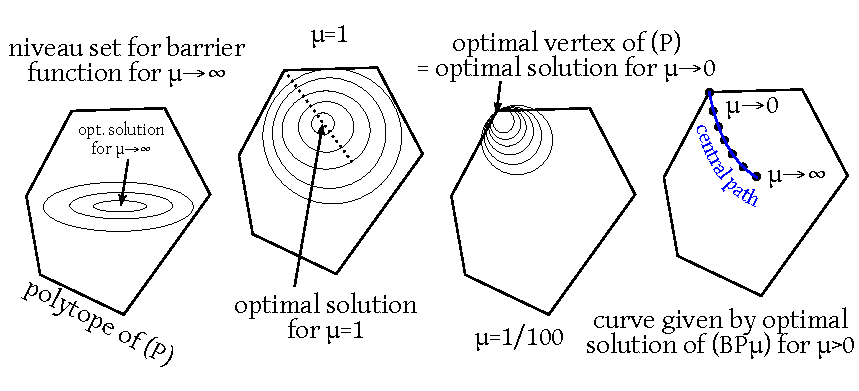
\includegraphics[width=0.7\textwidth]{img/10_inner_point_method_graphical_illustration.pdf}
		\caption{Graphical illustration}
		\label{img:graphical}
	\end{center}
\end{figure}

$(0)$ in vector notation:
\begin{align*}
	A^t y - z &= c \\
	Ax + w &= b \\
	XZ e &= \mu e \\
	YW e &= \mu e
\end{align*}

\emph{Question:} Is there always a solution of the corresponding barrier problem? \\
\emph{Answer:} No.

We consider two examples:
\begin{Example}
	\[ \max 0 \xrightarrow{\text{barrier function}} \max \mu \log x \qquad \mu > 0 \]
	subject to $x \geq 0$ does not have a finite optimum.
\end{Example}
\begin{Example}
	\[ \max -x \xrightarrow{\text{barrier function}} \max -x + \mu \log x \]
	(takes maximum with $x = \mu$) subject to $x \geq 0$ has a unique solution $x = 0$.
\end{Example}

\begin{theorem}
	\label{theorem:5.1}
	There exists a (finite) solution for the barrier problem if and only if the admissible set for the primal as well as the dual problem has a non-empty interior.
\end{theorem}

\begin{proof}
	\begin{description}
		\item[$\mathbf \implies$] trivial
		\item[$\mathbf \impliedby$] Assume there are inner points for $(P)$ and $(D)$, thus
			\begin{itemize}
				\item there exists $(\overline x, \overline w)$ an admissible solution for $(\overline P)$ with $\overline x > 0, \overline w > 0$ and
				\item there exists $(\overline y, \overline z)$ an admissible solution for $(\overline D)$ with $\overline y > 0, \overline z > 0$
			\end{itemize}
			so $(\overline x, \overline w, \overline y, \overline z) \in F^0$.
			Now consider $\overline z^t x + \overline y^t w$ for arbitrary admissible $(x, w)$ for $(\overline P)$.
			Insert slack variables:
			\[ \iff (A^t \overline y - c)^t x + \overline y^t (b - Ax) = b^t \overline y - c^t x \]
			Hence our target function is given as $c^t x = \overline z^t x - \overline y^t w + b^t \overline y$.

			$\to$ barrier problem of primal program

			\begin{align*}
				f(x, w) &= c^t x + \mu \sum_j \log x_j + \mu \sum_i \log w_i \\
					&= \sum_j \left(- \overline z_j x_j + \mu \log x_j\right) + \sum_i \left(-\overline y_i w_i + \mu \log w_i\right) + \underbrace{b^t \overline y}_{\text{constant}}
			\end{align*}
			Every summand in both sums is a function in only one variable.
			Those functions are all of form
			\[ \rho(\xi) = -\alpha \xi + \mu \cdot \log \xi \qquad \xi \in (0, \infty), \alpha > 0 \]
			Takes up a unique maximum for $\frac \mu\alpha$. Limit for $\xi \to \infty$ and $\to -\infty$
			\[ \SetDef{(x, w) \in \mathbb R^{n + m}}{f(x, w) \geq c} \]
			is bounded for constant $c$.

			\dateref{2019/04/09}
			% \begin{theorem}
			% 	The barrier problem has a finite solution if and only if $(\overline P)$ and $(\overline D)$ have strictly admissible solutions.
			% \end{theorem}

			\[ f(x, w) = c^t x + \mu \sum_j \log x_j + \mu \sum_i \log w_i \]
			\[ S \coloneqq \SetDef{(x, w) \in \mathbb R^{n + m}}{f(x, w) \geq c} \text{ bounded} \]
			Let $\overline f = f(\overline x, \overline w)$. $(\overline x, \overline w)$ is strictly admissible for $(\overline P$, $\overline x > 0$, $\overline w > 0$).
			Consider
			\[ \overline Q \coloneqq \SetDef{(x, w)}{Ax + w = b, x \geq 0, w \geq 0, f(x, w) \geq \overline f} \]
			Then $\overline Q \neq \emptyset$ because $(\overline x, \overline w) \in \overline Q$. Because $S$ is bounded, $\overline Q$ is bounded.
			Moreover, $\overline Q$ is closed. We show this the following way:
			\[ \overline Q = \SetDef{(x, w)}{Ax + w = b} \cap \SetDef{(x, w)}{x \geq 0, w \geq 0} \cap \SetDef{(x, w)}{f(x, w) \geq F} \]
			$\Set{f(x, w) \geq f}$ is the inverse image of $[\overline f, \infty)$ for the continuous function $f$, thus also closed.
			$\overline Q$ is the intersection of three closed set, thus closed itself.

			Thus, $\overline Q \subseteq R^{n + m}$ is compact.
			Hence, continuous functions on non-empty compact sets $\overline Q$ take up a maximum.

			$f$ takes up the maximum on $\SetDef{(x, w)}{x > 0, w > 0}$ because by definition of $\overline Q$, the maximum is taken up in a region with values $\geq \overline f$.

			Thus, the existence of a solution for the barrier problem is guaranteed.
			In the following, we will show uniqueness:
			\[ f(x, w) = c^t x + \mu \sum_j \log(x_j) + \mu \sum_i \log(w_i) \]
			\[ \frac{\partial f}{\partial x_j} = c_j + \frac{\mu}{x_j}  \qquad  \frac{\partial^2 f}{\partial x_j^2} = -\frac{\mu}{x_j^2} \qquad \frac{\partial f}{\partial x_j w_i} = 0 \]
			\[ \frac{\partial f}{\partial w_i} = \frac{\mu}{w_i} \qquad \frac{\partial^2 f}{\partial w_i^2} = -\frac{\mu}{w_i^2} \]
			\begin{itemize}
				\item[$\implies$] The Hessian matrix of $f$ is a diagonal matrix full of negative values on the diagonal ($f$ is strictly concave). Every critical point of $f$ is a maximum.
				\item[$\implies$] Furthermore here there can be at most one single critical point and if it exists, it represents a global maximum.
			\end{itemize}
			Thus uniqueness is given.
	\end{description}
\end{proof}

\begin{corollary}
	\label{corollary:5.2}
	If the admissible set of $(\overline P)$ (and accordingly $(\overline D)$) contains a strictly admissible set (thus has a non-empty interior) and is bounded, then the system (we call it $S$)
	\[ Ax + w = b \qquad A^t y - z = c \qquad XZe = \mu e \quad (x_j z_j = \mu \forall j) \qquad YWe = \mu e \quad (y_i w_i = \mu \forall i) \]
	For all $\varepsilon > 0$ there exists a unique solution ($x_\mu, w_\mu, y_mu, z_\mu)$.
\end{corollary}

\begin{proof}
	Follows from Theorem~\ref{theorem:5.1} and Lemma~\ref{lemma:5.3}, which will be proven in the practicals.
\end{proof}

\begin{Definition}[Null variable]
	\index{Null variable}
	A variable that takes up value $0$ in all admissible solutions of the linear program.
\end{Definition}

\begin{lemma}
	\label{lemma:5.3}
	If a linear program has admissible solutions and the set of admissible solutions is bounded,
	then the corresponding dual program has strictly admissible solutions.

	More specifically,
	\[ M_{\overline P} = \SetDef{(x, w)}{Ax + w = b, x \geq 0, w \geq 0} \qquad M_{\overline P} \neq \emptyset \text{ bounded} \]
	\[ M_{\overline D} = \SetDef{(y, z)}{A^t y - z = c, y, z \geq 0} \]
	$\exists (z, w) \in M_{\overline D}$ with $z, w > 0$.
\end{lemma}

\begin{Remark}[Equivalently and easier to prove]
	If a linear program has admissible solution and the dual problem has null variables,
	then the admissible set of the linear problem is unbounded.
\end{Remark}

\begin{Definition}
	\[ \SetDef{(x_\mu, w_\mu, y_\mu, z_\mu)}{(x_\mu, w_\mu, y_\mu, z_\mu) \text{ is solution of the system $S$ from above}, \mu > 0} \]
	is called \emph{central path}\index{Central path}.
\end{Definition}

\begin{Remark}
	Assuming that $(\overline P)$ and $(\overline D)$ has strictly admissible solutions (in the following, this is assumed), the central path is well-defined.
\end{Remark}

\begin{Remark}
	Fundamentals finished. Now we want to achieve algorithmic implementation.
	These are the basic steps of a primal-dual path traversal method.

	The method discussed here is a one-phase method.
	We begin with $(x, w) > 0$, but $(x, w)$ must not be admissible for $(\overline P)$.
	$(y, z) > 0$, \dots, $(y, z)$ for $(\overline D)$.

	Our goal is to solve $(\overline P)$ and $(\overline D)$ optimally.
	The method is a non-finite iteration process requiring a termination condition.
\end{Remark}

\begin{enumerate}
	\item[0.] Begin with an arbitrary $(x, w, y, z) > 0$
	\item[1.] Determine an appropriate value for $\mu$
	\item[2.] Determine the direction $(\triangle x, \triangle w, \triangle y, \triangle z)$ (here we use path point $(x_\mu, w_\mu, y_\mu, z_\mu)$ as guide)
	\item[3.] Determine the step size $\vartheta$ such that $(\tilde x, \tilde w, \tilde y, \tilde z) > 0$ with
		\begin{align*}
			\tilde x &\coloneqq x + \vartheta \cdot \triangle x \\
			\tilde w &\coloneqq w + \vartheta \cdot \triangle w \\
			\tilde y &\coloneqq y + \vartheta \cdot \triangle y \\
			\tilde z &\coloneqq z + \vartheta \cdot \triangle z
		\end{align*}
	\item[4.] Substitute $(x, w, y, z)$ by $(\tilde x, \tilde w, \tilde y, \tilde z)$.
\end{enumerate}

As long as the termination condition is not met, repeat steps 1--4.
But many details require further discussion.
l
\begin{Remark}[Direction determination (step 2)]
	Our goal is to determine $(\triangle x, \triangle w, \triangle y, \triangle z)$ such that $(x + \triangle x, w + \triangle w, y + \triangle y, z + \triangle z)$ lies in the neighborhood of point $(x_\mu, w_\mu, y_\mu, z_\mu)$ (point at the central path at this $\mu$).

	Insert $(x + \triangle x, w + \triangle w, y + \triangle y, z + \triangle z)$ into the central path system.

	\begin{align}
		A(x + \triangle x) + (w + \triangle w) &= b \label{eq1}\\
		A^t(y + \triangle y) - (z + \triangle z) &= c \label{eq2}\\
		(X + \triangle X)(Z + \triangle Z) e &= \mu e \label{eq3}\\
		(Y + \triangle Y)(W + \triangle W) e &= \mu e \nonumber
	\end{align}
	where the fourth equation belongs to \ref{eq3} and unknown variables are $\triangle x, \triangle y, \triangle X, \triangle Y, \triangle w, \triangle z, \triangle W$ and $\triangle Z$.
	Equations \ref{eq1} and \ref{eq2} are linear equation systems.

	Recall that,
	\[
		\triangle X = \begin{pmatrix}
			\triangle x_1 & & 0 \\
			& \ddots & \\
			0 & & \triangle x_n
		\end{pmatrix}
	\]
	\[ (x_j + \triangle x_j) (z_j + \triangle z_j) = \mu \forall j \]
	\[ (y_i + \triangle y_i) (w_i + \triangle w_i) = \mu \forall i \]
	\[ (x_j + \triangle x_j) (z_j + \triangle z_j) = x_j z_j + z_j \triangle x_j + x_j \triangle z_j + \triangle x_j \triangle z_j \]
	This is a non-linear term. To handle the non-linearity of the third expression, we apply the Newton method.

	The generic problem statement is:

	\emph{Given:} function $F: \mathbb R^n \to \mathbb R^n$ \\
	\emph{Find:} $\xi^* \in \mathbb R^n$ with $F(\xi^*) = 0$
	\[ F(\xi) = \begin{pmatrix} F_1(\xi) \\ \vdots \\ F_N(\xi) \end{pmatrix} \qquad \xi = \begin{pmatrix} \xi_1 \\ \vdots \\ \xi_N \end{pmatrix} \]

	The application looks as follows:
	Starting with $\xi \in \mathbb R^N$ with $F(\xi) \neq 0$, we determine $\triangle \xi$ and $\tilde\xi = \xi + \triangle \xi$ substitutes $\xi$.

	In the perfect setting, we have $F(\xi + \triangle \xi) = 0$ but for non-linear functions this is is a non-realistic goal in one step.
	Taylor approximation of $F$ up to terms of order $1$.
	\[ F(\xi + \triangle \xi) \approx F(\xi) + F'(\xi) \triangle \]
	Solve $F'(\xi) \triangle \xi = -F(\xi)$ and so on for the next point $\xi + \triangle \xi$ etc.
	\[
		F'(\xi) = \begin{bmatrix}
			\frac{\partial F_1}{\partial \xi_1} & \frac{\partial F_1}{\partial \xi_2} & \dots & \frac{\partial F_1}{\partial \xi_N} \\
			\frac{\partial F_2}{\partial \xi_1} & \dots & \dots & \vdots \\
			\vdots &  & \ddots & \\
			\frac{\partial F_N}{\partial \xi_1} & \frac{\partial F_N}{\partial \xi_2} & \dots & \frac{\partial F_N}{\partial \xi_N} \\
		\end{bmatrix}
	\]
	In our case:
	\[ \xi = \begin{pmatrix} x \\ y \\ w \\ z \end{pmatrix} \qquad F(\xi) = \begin{pmatrix} Ax + w - b \\ A^t y - z - c \\ XZ e - \mu e \\ YW e - \mu e \end{pmatrix} \]
	$I$ is the corresponding unit matrix. $0$ is the corresponding zero matrix.
	\[ F'(\xi) = \begin{pmatrix} A & 0 & I & 0 \\ 0 & A^t & 0 & -I \\ Z & 0 & 0 & X \\ 0 & W & Y & 0 \end{pmatrix} \]
	in block matrix notation.
	\[ \triangle \xi = \begin{pmatrix} \triangle x \\ \triangle y \\ \triangle w \\ \triangle z \end{pmatrix} \]
	As solution for $\triangle \xi$, we get the solution of
	\begin{align*}
		A \triangle x + \triangle w &= \rho \\
		A^t \triangle y - \triangle z &= \sigma \\
		Z \triangle x + X \triangle z &= \mu e - XZe \\
		W \triangle y + Y \triangle w &= \mu e - YWe
	\end{align*}

	\begin{align*}
		A \triangle x + \triangle w &= b - Ax - w \eqqcolon \rho & \text{primal residue} \\
		A^t \triangle y - \triangle z &= c - A^t y + z \eqqcolon \sigma & \text{dual residue}
		Z \triangle x + X \triangle z + \triangle X \triangle Z e &= \mu e - XZe \\
		W \triangle y + Y \triangle w + \triangle Y \triangle W e &= \mu e - YWe
	\end{align*}
	We want to apply linearization to the third and fourth equation.
	The omission of non-linear expressions and solving the linear equation system corresponds to the Newton step.
\end{Remark}

\begin{Remark}[About the choice of $\mathbf \mu$]
	If $\mu$ is chosen too large, then the danger is convergence to the analytical center of admissible sets, which is undesirable.
	If $\mu$ is chosen too small, the deviation from the central path can become too large (thus we are pushed to non-optimal marginal solutions).

	At the beginning, in general $(x, w, y, z)$ does not lie on the central path.
	There are various possibilities for the choice of $\mu$.
	For example, we could compute $x_j, z_j$ for some fixed $j$ and $w_i, y_i$ for some fixed $i$. Or
	\[ \mu = \frac{x^t z + y^t w}{n + m} \qquad \text{\enquote{Average value}} \]
	which gives the exact value if $(X, W, Y, Z)$ is on the central path. Also
	\[ \mu = \delta \cdot \frac{x^t z+ y^t w}{n + m} \qquad \delta \in (0, 1) \]
	In particular, $\delta = \frac1{10}$ was established as practical parameter.
\end{Remark}

\dateref{2019/04/29}

\begin{Revision}
	\[ \max c^t x \]
	\[ \text{s.t. } Ax + w = b; x, w \geq 0 \]

	\[ \min b^t y \]
	\[ \text{s.t. } A^t y - z = c; y, z \geq 0 \]

	\begin{align*}
		Ax + w &= b \\
		A^t y - z &= c \\
		XZe &= \mu e \\
		YWe &= \mu e \\
		X, W, Y, Z &\geq 0
	\end{align*}
	\[ X_j Z_j = \mu \forall j \qquad Y_i W_i = \mu \forall i \]

	\[ x, w, y, z \to (x + \theta \triangle x, w + \theta \triangle w, y + \theta \triangle y, z + \theta \triangle z) \]
	all components should stay positive (hence admissible and not on the boundary).

	Choice of $\mu$:
	\[ \mu = \triangle \frac{x^tz + y^tw}{n + m} \qquad \triangle \in (0, 1), \text{ e.g. } \triangle = \frac{1}{10} \]
\end{Revision}

By the choice of $\theta$ (step size),
\begin{align*}
	x_j + \theta \triangle x_j &> 0 \to \frac1\theta > -\frac{\triangle x_j}{x_j} \forall j \\
	z_j + \theta \triangle z_j &> 0 \\
	w_i + \theta \triangle w_i &> 0 \\
	y_i + \theta \triangle y_i &> 0 \\
\end{align*}
\[ \frac{1}{\theta^*} = \max_{i,j} \Set{-\frac{\triangle x_j}{x_j}, -\frac{\triangle z_j}{z_j}, \frac{\triangle w_i}{w_i}, \frac{\triangle y_i}{y_i}} \]
To avoid contact with boundary, we choose $\theta$ such that
\[ \theta = \min\Set{r \Set{\max_{i, j} \Set{-\frac{\triangle x_j}{x_j}, -\frac{\triangle z_j}{z_j}, \frac{\triangle w_i}{w_i}, \frac{\triangle y_i}{y_i}}}^{-1}, 1} \]
Thus $r < 1$, but close to $1$.

\begin{Revision}[Linear Newton system]
	$\triangle x, \triangle y, \triangle z, \triangle w$ as solution of
	\begin{align*}
		A \triangle x + \triangle w &= \triangle \\
		A^t \triangle y - \triangle z &= \sigma \\
		Z \triangle x + X \triangle z &= \mu e - XZe \\
		W \triangle y + Y \triangle w &= \mu e - ZWe \\
	\intertext{with}
		\rho &= b - Ax - w \\
		\sigma &= c - A^t y + z
	\end{align*}
\end{Revision}

The algorithm is completely specified.
The analysis remains to be done.

Measuring progress:
\begin{enumerate}
	\item Measuring primal admissibility
	\item Measuring dual admissibility
	\item Performance (size of duality gap) and accordingly complement notion
\end{enumerate}
Use $\rho = b - Ax - w$, $\rho = c - A^t y + z$ and $\gamma = z^t x + y^t w$.

\subsubsection{Progress in one iteration}
\begin{enumerate}
	\item Measuring primal admissibility
		\[ \hat g = b - A \hat x - \hat w = \underbrace{b - Ax - w}_{\rho} - \theta (A\triangle x + \triangle w) \]
		where $A\triangle x + \triangle w = \rho$ according to the Linear Newton system. Hence,
		\[ \hat g = b - A \hat x - \hat w = (1 - \theta) \rho \]
	\item Analogously, we get,
		\[ \hat \sigma = c - A^t \hat y + \hat z = \dots = (1 - \theta) \sigma \]
	\item
		\begin{align}
			\hat y &= \hat z^t + \hat x + \hat y^t \hat w \label{num}\\
				&= (z + \theta \triangle z)^t (x + \theta \triangle x) + (y + \theta \triangle y)^t + (w + \theta \triangle w) \nonumber\\
				&= \underbrace{z^t x + y^t w}_{\gamma} + \theta (z^t \triangle x + \triangle z^t x + y^t \triangle w + \triangle y^t w)
				+ \theta^2 (\triangle z^t \triangle x + \triangle y^t \triangle w) \nonumber
		\end{align}
		where $\triangle z^t \triangle x + \triangle y^t \triangle w = (A^t \triangle y - \sigma)^t \triangle x + \triangle y^t (\rho - A \triangle x) = \triangle y^t \rho - \sigma^t \triangle x$.
		By the Linear Newton system, we have,
		\begin{align*}
			z^t \triangle x + \triangle z^t x &= e^t \left(Z \triangle x + X \triangle z\right) \\
				&= e^t \left(\mu e - ZXe\right) = \mu n - z^t x
		\end{align*}
		Analogously,
		\begin{align*}
			y^t \triangle w + \triangle y^t w &= e^t \left(Y \triangle w + W \triangle y\right) + e^t \left(\mu e - YWe\right) = \mu m - y^t w
		\end{align*}
		\begin{align*}
			\triangle z^t \triangle x + \triangle y^t \triangle w
				&= (A^t \triangle y - \sigma)^t \triangle x + \triangle y^t (\rho - A \triangle x) \\
				&= \triangle y^t \rho - \sigma^t \triangle x
		\end{align*}
		Thus, by \eqref{num},
		\[ \hat y = \underbrace{z^t x + y^t w}_{\gamma} + \theta\underbrace{\left(\mu(n + m) - (z^t x + y^t w)\right)}_{\delta \gamma} + \theta^2 \left(\triangle y^t \rho - \sigma^t \triangle x\right) \]
		So, $\hat\gamma = (1 - (1 - \delta) \theta) \gamma + \theta^2 \left(\triangle y^t \rho - \sigma^t \triangle x\right)$.
		We continue using estimates.

		The following special case of Hölder's inequality is helpful:
		\[ \Abs{v^t u} = \Abs{\sum_j v_j u_j} \leq \sum_j \Abs{v_j} \Abs{u_j} \leq \left(\max_{j} \Abs{v_j}\right) \cdot \sum_j \Abs{u_j} = \Norm{v}_\infty \cdot \Norm{u}_1 \]

		In our case, we get:
		\begin{align*}
			\Abs{\triangle y^t \rho} &\leq \Norm{\rho}_1 \Norm{\triangle y}_\infty \\
			\Abs{\sigma^t \triangle x} &\leq \Norm{\sigma}_1 \cdot \Norm{\triangle x}_{\infty} \\
		\intertext{Hence,}
			\hat y &\leq (1 - (1 - \delta) \theta) \gamma + \theta \left(\Norm{\rho}_1 \cdot \Norm{\theta \triangle y}_\infty + \Norm{\sigma}_1 \cdot \Norm{\theta \triangle x}_\infty\right)
		\end{align*}
		By choice of $\theta$, 
		\[ \theta \leq \frac{x_j}{\Abs{\triangle x_j}} \text{ for all } j \]
		\[ \to \Norm{\theta \triangle x}_{\infty} \leq \Norm{x}_{\infty} \]
		Analogously, $\Norm{\theta \triangle g}_{\infty} \leq \Norm{y}_\infty$.
		Assume $\Norm{x}_{\infty}$ and $\Norm{y}_\infty$ are bounded by above, then $\exists M \in \mathbb R: \Norm{x}_{\infty} \leq M$ and $\Norm{y}_\infty \leq M$ ($M$ can be very large). Thus,
		\[ \hat y \leq (1 - (1 - \delta) \theta) \gamma + \theta (M \Norm{\rho}_1 + M \cdot \Norm{\sigma}_1) \]
\end{enumerate}

\subsubsection{About the termination condition}

Let $\varepsilon > 0$ be a small tolerance parameter and $0 < M < \infty$ a large tolerance parameter.
\begin{itemize}
	\item If $\Norm{x}_{\infty} > M$ is true at some point, then STOP with error \enquote{(P) is unbounded} ($M$ must be chosen sufficiently large!)
	\item If $\Norm{y}_{\infty} > M$ is true at some point, then STOP with error \enquote{(D) is unbounded}
	\item If $\Norm{\rho}_1 < \varepsilon$ (sufficiently primaly admissible), $\Norm{\sigma}_1 < \varepsilon$ (sufficiently dually admissible) and $\gamma < \varepsilon$ (suffienciently optimal), then STOP and return current $x$ (i.e. $(x, z)$) and current $y$ (i.e. $(y, w)$) as optimal solution of (P) and accordingly (D).
\end{itemize}

\subsubsection{Relation of $\gamma$ and the performance of the duality gap}

\begin{align*}
	\gamma &= z^t x + y^t w
		= (\sigma + A^t y - c)^t x + y^t (b - Ax - \rho) \\
		&= \underbrace{b^t y - c^t x}_{\text{duality gap}} - \sigma^t x - \rho^t y \\
	\Abs{b^t y - c^t x} &\leq \gamma + \Abs{\sigma^t x} + \Abs{y^t \rho} \\
		&\leq \gamma + \Norm{\rho}_1 \cdot \Norm{x}_{\infty} + \Norm{\rho}_1 \Norm{y}_\infty
\end{align*}
So, if $\gamma, \Norm{\sigma}_1, \Norm{\rho}_1$ are sufficiently small (and $\Norm{x}_\infty$ and $\Norm{y}_{\infty}$ are sufficiently large), then the duality gap is sufficiently small.

You should not expect that the duality gap becomes sufficiently small before $x$ and $y$ are almost admissible ($\Norm{\sigma_1}$ and $\Norm{\rho}_1$ sufficiently small) (this is also confirmed in numerical experiments).

\subsubsection{Analysis of progress over multiple iterations}

Denote $\rho^{(k)}, \sigma^{(k)}, x^{(k)}, y^{(k)}, z^{(k)}, w^{(k)}, \gamma^{(k)}, \theta^{(k)}$, et cetera denote the corresponding value in iteration $k$ (iteration 0 defines the initial values).

\begin{theorem}
	\label{theorem:5.4}
	Assume $\exists t \in \mathbb R, t > 0, M \in \mathbb R, M < \infty$ and $K \in \mathbb N$ such that
	\[ \theta^{(k)} \geq t \qquad \Norm{x^{(k)}} \leq M \qquad \Norm{y^{(k)}} \leq M \]
	is true for all $k \leq K$. Then $\exists \hat M < \infty$ such that
	\begin{align*}
		\Norm{\rho^{(k)}}_1 &\leq (1 - t)^k \Norm{\rho^{(0)}}_1 \\
		\Norm{\sigma^{(k)}}_1 &\leq (1 - t)^k \Norm{\sigma^{(0)}}_1 \\
		\gamma^{(k)} &\leq (1 - \tilde t)^k \cdot \hat M
	\end{align*}
	for all $k \in K$ with $\tilde t \coloneqq (1 - \delta)$.
\end{theorem}

\begin{proof}
	By analysis of the progress in one iteration, we get:
	\begin{align*}
		\Norm{g^{(k)}}_1 &\leq (1 - t) \cdot \Norm{g^{(k-1)}}_1 \leq \dots \leq (1 - t)^k \cdot \Norm{\rho^{(0)}}_1 \\
		\Norm{\sigma^{(k)}}_1 &\leq (1 - t) \Norm{\sigma^{(k-1)}}_1 \leq \dots \leq (1 - t)^k \Norm{\sigma^{(0)}}_1
	\end{align*}
	More difficult for $\gamma(k)$, we get
	\[ \gamma(k) \leq (1 - t(1 - \delta)) \gamma^{(k - 1)} + M (1 - t)^{k-1} \left(\Norm{\rho^{(0)}}_1 + \Norm{\rho^{(0)}}_1\right) \]
	\[ = (1 - \tilde t) \gamma^{(k-1)} + \tilde M (1 - t)^{(k - 1)} \text{ with } \tilde M = M(\Norm{\rho^{(0)}}_1 + \Norm{\sigma^{(0)}}_1) \]
	\[ \leq (1 - \tilde t)\left((1 - \tilde t) \gamma^{(k-2)} + \tilde M (1 - t)^{k-2}\right) \]
	\[ = (1 - \tilde t)^2 \gamma^{k-2} + \tilde M (1 - t)^{k-1} \cdot \left(\frac{1 - \tilde t}{1 - t} + 1\right) \]
	\[ \vdots \]
	\[ \leq (1 - \tilde t)^k \gamma^{(0)} + \tilde M (1 - t)^{k-1} \left[\left(\frac{1 - \tilde t}{1 - t}\right)^{k-1} + \dots + \frac{1 - \tilde t}{1 - t} + 1\right] \]
	gives a geometrical sum. Hence,
	\[ = (1 - \tilde t)^k \gamma^{(0)} + \tilde M \cdot (1 - t)^{k-1} \cdot \left(1 - \left(\frac{1 - \tilde t}{1 - t}\right)^k\right) \left(1 - \frac{1 - \tilde t}{1 - t}\right)^{-1} \]
	\[ = (1 - \tilde t)^k \cdot \gamma^{(0)} + \tilde M \left((1 - \tilde t)^k - (1 - t)^k\right)(t - \tilde t)^{-1} \]
	\[ \leq (1 - \tilde t)^k \cdot \gamma^{(0)} + \tilde M \left(1 - \tilde t\right)^k \cdot (\delta t)^{-1} \]
	\[ = (1 - \tilde t)^k \cdot (\gamma^{(0)} + \tilde M \cdot (\delta t)^{-1}) \]
\end{proof}

\begin{Remark}[Remark about Theorem~\ref{theorem:5.4}]
	Theorem~\ref{theorem:5.4} is a constrained convergence result, because the assumption $\theta^{(n)} \geq t \forall k \leq K$ was made such that the step size of $\theta$ is path bounded. The latter can be achieved by a modification of the algorithm and a proper choice of an initial solution. Details can be looked up in literature.
\end{Remark}

\begin{Remark}
	Consider that factor $(1 - t)$ per iteration for $\rho$ and $\sigma$ and factor $(1 - \tilde t)$ for $\gamma$.
	Recognize that in practice, it can be shown that the dual gap converges slower than primal and dual inadmissibility.
\end{Remark}

For practice, a lot of implementation details need to be discussed, but we won't do it in class.

By convergence analysis we get that the primal-dual path traversal method leads to a method that can determine an almost-optimal pair $(x, y)$ in polynomial time. The termination condition is left to be discussed.

\dateref{2019/04/30}

\section{Nonlinear optimization without constraints}
\subsection{Basic terminology}

We consider functions of $\mathbb R^n \to \mathbb R$.

\begin{definition}[minimum, maximum]
	\index{Global minimum}
	\index{Local minimum}
	\index{Strict global minimum}
	\index{Strict local minimum}
	Function $f: \mathbb R^n \to \mathbb R$ has a
	\begin{description}
		\item[global minimum] in $x^* \in \mathbb R$ if $f(x^*) \leq f(x) \forall x \in \mathbb R^n$
		\item[strict global minimum] in $x^* \in \mathbb R$ if $f(x^*) < f(x) \forall x \in \mathbb R^n \setminus \Set{x^*}$
		\item[local minimum] in $x^* \in \mathbb R$ if $\exists \varepsilon > 0$ such that $f(x^*) \leq f(x) \forall x \in \mathcal U_\varepsilon(x^*)$
		\item[strict local minimum] if $\exists \varepsilon > 0$ such that $f(x^*) < f(x) \forall x \in U_\varepsilon(x^*) \setminus \Set{x^*}$
	\end{description}
	Analogously for maximum/maxima.

	\index{Minimizer}
	The minimum/maximum $x^*$ satisfying the (strict/weak local/global) criteria, is also called (local/global) \emph{minimizer}.
\end{definition}

\begin{Remark}
	Every global minimum is also a local minimum, but not vice versa. \\
	For convex functions, the two definitions collapse. \\
	For simplicity, we always consider minimization problems.
\end{Remark}

\begin{Remark}
	The typical goal in the field of non-linear optimization (and thus also what software on this field typically does), is determination of local optima (min or max) or potential candidates. Determination of global optima is significantly more difficult. Thus a separate field of global optimization was established.
\end{Remark}

\begin{Example}
	A typical problem in non-linear unconstrained optimzation is: given $f$, find local minima of $f$.
	\[ \min_{x \in \mathbb R^n} f(x) \]
	This is different from non-linear optimzation \emph{with} constraints:
	Given $f$, find $x \subset \mathbb R^n$
	\[ \min f(x) \qquad \text{s.t. } x \in X \]
\end{Example}

One important aspect are optimality criteria (criteria for local optima).
In the following, we assume that $f$ is differentiable.

\begin{definition}
	\index{Stationary point}
	Let $f: \mathbb R^n \to \mathbb R$ be continuously differentiable. Then we call $x^* \in \mathbb R^n$ \emph{stationary point} of $f$ if $\nabla f(x^*) = 0$.
\end{definition}

\begin{theorem}
	\label{theorem:2.1.1}
	Let $f: X \to \mathbb R$ be a continously differentiable function and let $X \subseteq \mathbb R^k$ be an open set. If $x^* \in X$ is a local minimum of $f$ (on $X$), then $\nabla f(x^*) = 0$, thus $x^*$ is a stationary point on $f$.
\end{theorem}

\begin{proof}
	Suppose $x^*$ is a local minimum of $f$ with $\nabla f(x^*) \neq 0$.
	Then there exists $d \in \mathbb R^n$ with $(\nabla f(x^*))^t d < 0$ (e.g. choose $d = -\nabla f(x^*) \neq 0$).
	Because $f$ is continuously differentiable by assumption, the directional derivative of $f$ in $x^*$ in direction $d$ satisfies:
	\[ f'(x^*, d) = \lim_{t \to 0} \frac{f(x^* + td) - f(x^*)}{t} = \left(\nabla f(x^*)\right)^t d < 0 \]
	\[ \exists \overline{t} > 0: x^* + td \in X \text{ and } \frac{f(x^* + td) - f(x^*)}{t} < 0 \forall t \in (0, \overline{t}] \]
	\[ f(x^* + td) < f(x^*) \forall t \in (0, \overline t] \]
	This is a contradiction to $x^*$ as a local minimum.
\end{proof}

\begin{Remark}
	\begin{enumerate}
		\item The approach within the proof and the relevance of the directional derivative will reoccur in our algorithmic considerations. Keyword \enquote{line search algorithms}.
		\item The condition $\nabla f(x^*) = 0$ is not sufficient for existence of a local minimum (e.g. such a $x^*$ can also be local maximum of $f$ or neither nor).
	\end{enumerate}
\end{Remark}

\begin{theorem}
	\label{theorem:2.1.2}
	Let $X \subseteq \mathbb R^n$ be an open set and let $f: X \to \mathbb R^n$ be two times differentiable.
	If $x^*$ is a local minimum of $f$ (on $X$), then the Hessian matrix $\nabla^2 f(x^*)$ of $f$ in $x^*$ is positive definite.

	This is a necessary condition of second order.
\end{theorem}

\begin{proof}
	Assume $x^*$ is a local minimum, but $\nabla^2 f(x^*)$ is not positive semi-definite, thus $\exists d \in \mathbb R^n$ with $d^t \nabla^2 f(x^*) d < 0$.

	By Theorem~\ref{theorem:2.1.1} ($\to \nabla f(x^*) = 0$) together with Taylor's theorem, we get that for all sufficiently small $t > 0$,
	\[ f(x^* + td) = f(x^*) + \frac12 t^2 d^t \nabla^2 f(\xi_t) d \text{ where } \xi_t = x^* + \vartheta _t td \text{ for some } \vartheta_t \in (0, 1) \]
	Using continuity, we can conclude that $\exists \overline{t} > 0$ such that $f(x^* + td) < f(x^*) \forall t \in (0, \overline{t}]$. This is a contradiction to $x^*$ being a local minimum.
\end{proof}

\begin{Remark}
	Also these two criteria are insufficient for the existence of a local minimum.
	\begin{Example}
		$n = 2$. $f(x) = x_1^2 - x_2^4$, $x^* = (0, 0)$.
	\end{Example}
\end{Remark}

\begin{theorem}
	\label{theorem:2.1.3}
	Let $X \subseteq \mathbb R^n$ be open and let $f: X \to \mathbb R$ be two times differentiable. If
	\begin{enumerate}
		\item $\nabla f(x^*) = 0$
		\item $\nabla^2 f(x^*)$ positive definite
	\end{enumerate}
	then $x^*$ is a strict local minimum of $f$ (on $X$).

	This is a sufficient optimality criterion of second order.
\end{theorem}

\begin{proof}[Proof sketch]
	It can be shown that the second condition yields,
	\[ \exists \mu > 0: d^t \nabla^2 f(x^*) d \geq \mu d^t d \forall d \in \mathbb R^n \]
	By Taylor's theorem, $\forall d \in \mathbb R^n$, that are sufficiently close to the zero-vector, that
	\[ f(x^* + td) = f(x^*) + \nabla f(x^*)^t d + \frac12 d^t \nabla^2 f(\xi_d) d \]
	with $\xi_d = x^* + \vartheta_d$ and $\vartheta_d \in (0, 1)$.
	By the first condition and the Cauchy-Schwarz inequality, we get
	\begin{align*}
		f(x^* + d) &= f(x^*) + \frac12 d^t \nabla^2 f(x^*) d + \frac12 d^t \left(\nabla^2 f(\xi_d) - \nabla^2 f(x^*)\right) d \\
			&\geq f(x^*) + \frac12 \left(\mu - \Norm{\nabla^2 f(\xi_d) - \nabla^2 f(x^*)}\right) \Norm{d}^2
	\end{align*}
	\[ \implies f(x^* + d) > f(x^*) \forall d \neq 0 \text{ sufficiently close to } 0 \]
	\[ \implies x^* \text{ is a strict local minimum} \]
\end{proof}

\begin{Remark}
	The criterion above is not sufficient.
	\begin{Example}
		$n = 2$, $f(x) = x_1^2 + x_2^4$, $x^* = (0, 0)$
	\end{Example}
\end{Remark}

\subsection{Convex functions}

This is a brief, introductory section.
\begin{Definition}
	\index{Convexity}
	$X \subseteq \mathbb R^n$ is called \emph{convex} if $\forall x, y \in X \forall \lambda \in [0, 1]: \lambda x + (1 - \lambda) y \in X$
\end{Definition}

\begin{Definition}
	Let $X \subseteq \mathbb R^n$ be convex.
	A function $f: X \to \mathbb R$ is called
	\begin{description}
		\item[convex on $X$] if $\forall x, y \in X \forall \lambda \in [0, 1]: f(\lambda x + (1 - \lambda) y) \leq \lambda f(x) + (1 - \lambda) f(y)$
		\item[strictly convex on $X$] if $\forall x, y \in X \forall \lambda \in (0, 1): x \neq \implies f(\lambda x + (1 - \lambda) y) < \lambda f(x) + (1 - \lambda) f(y)$
		\item[uniformly convex on $X$] if $\exists \mu > 0: f(\lambda x + (1 - \lambda) y) + \mu \lambda (1 - \lambda) \Norm{x - y}^2 \leq \lambda f(x) + (1 - \lambda) f(y) \forall x, y \in X \forall \lambda \in (0, 1)$.
			$\mu$ is also called \emph{modulo}.\index{Modulo of uniform convexity}
	\end{description}
\end{Definition}

\begin{figure}[t]
	\begin{center}
		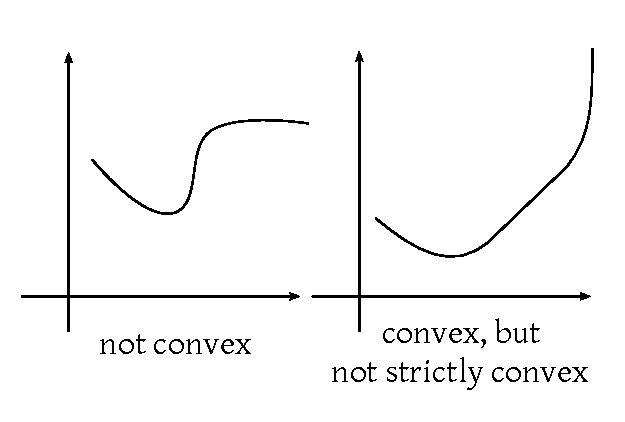
\includegraphics{img/20_strict_convexity.pdf}
		\caption{Convexity versus strict convexity}
		\label{img:convexity}
	\end{center}
\end{figure}

In case of a convex function, no point of a segment between two points $(x, f(x)), (y, f(y)) \in \mathbb R^{n+1}$ lies below the graph of $f$.

\begin{Remark}
	Every strict convex function is convex.
	Every uniform convex function is strict convex.
	The other directions do not hold in general.
\end{Remark}

\begin{Example}
	\begin{itemize}
		\item $f(x) = x$ is convex
		\item $f(x) = e^x$ is strictly convex, not uniform
		\item $f(x) = x^2$ is uniformly convex
	\end{itemize}
	On the opposite side, $x^4$ is strictly convex, but not uniformly convex.
	For the special case of quadratic functions, the following result can be shown easily:

	Let $f: \mathbb R^n \to \mathbb R$ with $f(x) = \frac12 x^t Qx + c^t x + \gamma$ with $Q$ as symmetric $n \times n$ matrix over $\mathbb R$, $c \in \mathbb R^n$, $\gamma \in \mathbb R$. Then,
	\begin{enumerate}
		\item $f$ is convex iff $Q$ is positive semidefinite
		\item $f$ is strictly convex iff $f$ is uniformly convex iff $Q$ is positive definite
	\end{enumerate}
\end{Example}

TODO

\dateref{2019/05/06}

Our next goal are characterizations (of first or second order) for
\begin{itemize}
	\item convex
	\item strict convex
	\item uniform convexity
\end{itemize}

\begin{theorem}
	\label{theorem:5.2.1}
	Let $X \subseteq \mathbb R^n$ open and convex and $f: X \to \mathbb R$ is continuously differentiable.
	Then
	\begin{enumerate}
		\item $f$ is convex (on $X$) iff $f(x) - f(y) \geq (\triangle f(y))^t (x - y) \forall x, y \in X$
		\item $f$ is strictly convex (on $X$) iff $f(x) - f(y) > (\triangle f(y))^t (x - y) \forall x, y \in X$
		\item $f$ is uniformly convex (on $X$) iff $f(x) - f(y) \geq (\nabla f(y))^t (x - y) + \mu \Norm{x - y}^2 \forall x, y \in X$
	\end{enumerate}
\end{theorem}

\begin{proof}
	\begin{description}
		\item[(1) and (2)] are left as an exercise for the reader
		\item[(3)] Let $f$ be uniformly convex.
			$\forall x, y \in X \forall \lambda \in (0, 1)$ for some $\mu > 0$,
			\[ f(y + \lambda (x - y)) \leq \lambda f(x) + (1 - \lambda) f(y) - \mu \lambda (1 - \lambda) \Norm{x - y}^2 \]
			\[ \frac{f(y + \lambda(x - y)) - f(y)}{\lambda} \leq f(x) - f(y) - \mu(1 - \lambda) \Norm{x - y}^2 \]
			For $\lambda \to 0^+$, we get (by continuous differentiability of $f$)
			\[ (\nabla f(y))^t (x - y) = \lim_{\lambda \to 0^+} \frac{f(y + \lambda(x - y)) - f(y)}{\lambda} \leq f(x) - f(y) - \mu\Norm{x - y}^2 \]
			Thus, the third property follows.
	\end{description}
	The rest of the proof is left as an exercise to the reader.
\end{proof}

\begin{Definition}
	Let $X \subseteq \mathbb R^n$. Consider $F: X \to \mathbb R^n$. Then $F$ is called
	\begin{enumerate}
		\item monotonous (on $X$) if $(X - y)^t (F(x) - F(y)) \geq 0 \forall x, y \in X$
		\item strictly monotonous (on $X$) if $(X - y)^t (F(x) - F(y)) > 0 \forall x, y \in X$
		\item uniformly monotonous (on $X$) if $(x - y)^t (F(x) - F(y)) \geq \mu \Norm{x - y}^2 \forall x, y \in X$
	\end{enumerate}
\end{Definition}

\begin{Remark}
	For $n = 1$, this corresponds to scalar functions and the usual notion of monotonicity.
\end{Remark}

\begin{theorem}
	\label{theorem:5.2.2}
	Let $X \subseteq \mathbb R^n$ be open and convex and let $f: X \to \mathbb R$ be continuously differentiable. Then
	\begin{enumerate}
		\item $f$ is convex (on $X$) iff $\nabla f$ is monotonous
		\item $f$ is strictly convex (on $X$) iff $\nabla f$ is strictly monotonous
		\item $f$ is uniformly convex (on $X$) iff $\nabla f$ is uniformly monotonous
	\end{enumerate}
\end{theorem}

\begin{theorem}
	\label{theorem:5.2.3}
	Let $X \subseteq \mathbb R^n$ be open and convex and let $f: X \to \mathbb R$ be two times differentiable ($\to \nabla f$ is continuously differentiable). Then
	\begin{enumerate}
		\item $f$ is convex (on $X$) iff $\nabla^2 f(x)$ is positive semidefinite $\forall x \in X$
		\item $f$ is strictly convex (on $X$) \emph{if} $\nabla^2 f(x)$ is positive definite $\forall x \in X$
		\item $f$ is uniformly convex (on $X$) iff $\nabla^2 f(x)$ is uniformly positive definite on $X$, thus
			\[ \exists \mu > 0: d^t \nabla^2 f(x) d \geq \mu \Norm{d}^2 \forall x \in X \forall d \in \mathbb R^n \]
	\end{enumerate}
\end{theorem}

\begin{proof}
	Properties (1) and (2) are left as an exercise to the reader. We prove (3):
	\begin{description}
		\item[Direction $\implies$] 
			Only property 3 is new to us. Let $f$ be uniformly convex. Use Theorem~\ref{theorem:5.2.2}~(3). So $\nabla f$ is uniformly monotonous. By appropriately chosen $\mu > 0$, we get
			\begin{align*}
			  d^t \nabla^2 f(x) d &= d^t \lim_{t\to0} \frac{\nabla f(x + td) - \nabla f(x)}{t}
			  	= \lim_{t\to0} \frac{td^t(\nabla f(x + td) - \nabla f(x))}{t^2} \\
			  	&\geq \lim_{t\to0} \frac{1}{t^2} \mu \Norm{td}^2 
			  	= \mu \Norm{d}^2 \qquad\forall x \in X, d \in \mathbb R^n
			\end{align*}
			So, $\nabla^2 f(x)$ is uniformly positive definite.
		\item[Direction $\impliedby$]
			Let the third property be true. By the mean value theorem of differential calculus (in integral form),
			we get
			\begin{align*}
				(x - y)^t (\nabla f(x) - \nabla f(y)) &= \int_0^1 (x - y)^t \nabla^2 f(y + \alpha(x - y)) (x - y) \, d\alpha \\
					&\geq \mu \int_0^1 \Norm{x - y}^2 \, d\alpha = \mu \Norm{x - y}^2 \\
					&\implies \nabla f \text{ is uniformly monotonous on } X \\
					&\xRightarrow{\text{Theorem~\ref{theorem:5.2.2}~(3)}} f \text{ is uniformly convex on } X
			\end{align*}
	\end{description}
\end{proof}

\begin{Remark}
	To verify that $\nabla^2 f(x)$ is 
	\begin{description}
		\item[positive semidefinite] use $\forall \lambda \in \operatorname{spec}(\nabla^2 f(x)): \lambda \geq 0$
		\item[positive definite] use $\forall \lambda \in \operatorname{spec}(\nabla^2 f(x)): \lambda > 0$
		\item[uniformly positive definite] use $\forall \lambda \in \operatorname{spec}(\nabla^2 f(x) - \mu I): \lambda \geq 0$
	\end{description}
	Thus all eigenvalues of $\nabla^2 f(x)$ are greater-equal to $\mu$.
	Recognize that constant $\mu$ is independent of $x$.
	Thus the eigenvalue of $0$ is negatively bounded.
\end{Remark}

\begin{Remark}[Remark about (2)]
	$f(x) = x^4$ is strictly convex but $\nabla^2 f(x) = f''(x) = 12x^2$.
	$f''(0) = 0$, so $f$ is only positive semidefinite.
	There is only one direction in (2).
\end{Remark}

Our goal is to establish a result about the existence of a minimum.

\begin{Definition}
	Let $f: \mathbb R^n \to \mathbb R$
	\[ \mathcal L(\tilde x) = \SetDef{x \in \mathbb R^n}{f(x) \leq f(\tilde x)} \]
	defines a \emph{level set}\index{Level set}\dt{Niveaumenge}.
\end{Definition}

\begin{lemma}
	\label{lemma:5.2.4}
	Let $f: \mathbb R^n \to \mathbb R$ be continuously differentiable.
	Let $\tilde x \in \mathbb R^n$ with $\mathcal L(\tilde x)$ is convex and let $f$ be uniformly convex on $\mathcal L(\tilde x)$.

	Then $\mathcal L(\tilde x)$ is compact.
\end{lemma}

\begin{proof}
	$\mathcal L(\tilde x) \neq \emptyset \implies \exists x \in \mathcal L(\tilde x)$.
	Because $f$ is uniformly convex on $\mathcal L(\tilde x)$, we get (by $X = \frac12$ and appropriate $\mu > 0$)
	\begin{align*}
		\frac14 \mu \Norm{x - \tilde x}^2
			&\leq \frac12 \left(\frac12 f(x) - f(\tilde x)\right) - \left(f(\frac12(x + \tilde x)) - f(\tilde x)\right) \\
			&\leq -\left(f(\frac12(x + \tilde x)) - f(\tilde x)\right) \\
			&\leq -\frac12 \nabla f(\tilde x)^t (x - \tilde x) \\
			&\leq \frac12 \Norm{\nabla f(\tilde x)} \Norm{x - \tilde x}
	\end{align*}
	Thus $\Norm{x - \tilde x} \leq c$ with $c = \frac{2 \Norm{\nabla f(\tilde x)}}{\mu}$ (a constant independent of $x$) for all $x \in \mathcal L(\tilde x)$.

	Thus $\mathcal L(\tilde x)$ is bounded. Because $f$ is continuous, $\mathcal L(\tilde x)$ is closed.
	So $\mathcal L(\tilde x)$ is compact.
\end{proof}

\begin{Remark}
	Assume $f$ to be uniformly convex on entire $\mathbb R^n$ or only on a convex set $X$, that contains $\mathcal L(\tilde x)$.
	Then the convexity of $\mathcal L(\tilde x)$ follows immediately and we can omit the explicit precondition $\mathcal L(\tilde x)$.
\end{Remark}

\begin{theorem}
	\label{theorem:5.2.5}
	Let $f: \mathbb R^n \to \mathbb R$ be continuously differentiable and let $X \subseteq \mathbb R^n$ be convex.
	We consider the optimization problem (P) $\min_{x \in X} f(x)$. Then
	\begin{enumerate}
		\item If $f$ is convex on $X$, then the solution set of (P) is convex (potentially empty)
		\item If $f$ is strictly convex on $X$, then (P) has at most one solution.
		\item If $f$ is uniformly convex on $X$ and $X \neq \emptyset$ and $X$ is closed (e.g. for $X = \mathbb R^n$), then (P) has exactly \emph{one} solution
	\end{enumerate}
\end{theorem}

\begin{Remark}
	The third property illustrates the particular significance of the class of convex, strictly convex and uniformly convex functions in non-linear optimization.
\end{Remark}

\begin{proof}
	\begin{enumerate}
		\item Let $\bar x$ and $\bar{\bar x}$ be solutions of (P) with $\bar x, \bar{\bar x} \in X$.
		\[ f(\bar x) = f(\bar{\bar x}) = \min_{x \in X} f(x) \]
		For $\lambda \in (0, 1)$, we have $\lambda \bar{x} + (1 - \lambda) \bar{\bar x} \in X$, because $X$ is convex.

		Because $f$ is convex,
		\begin{align*}
			f(\lambda \bar{x} + (1 - \lambda) \bar{\bar x})
				&\leq \lambda f(\bar x) + (1 - \lambda) f(\bar{\bar x}) \\
				&= f(\bar{x}) = \min_{x \in X} f(x) \\
				&\implies \text{ also } \lambda \bar{x} + (1 - \lambda) \bar{\bar x} \text{ is solution of } (P)
		\end{align*}
		\item Assume there are 2 different solutions $\bar x$ and $\bar{\bar x}$ with $\bar x \neq \bar{\bar x}$.
			For $\lambda \in (0, 1)$,
			\[ f(\lambda \bar x + (1 - \lambda) \bar{\bar x}) < \lambda f(\bar{x}) + (1 - \lambda) f(\bar{\bar x}) = f(\bar x) = \min_{x \in X} f(x) \]
			as $f$ is strictly convex.
			This is a contradiction to $\bar{x}$ and $\bar{\bar x}$ as solutions of (P).
		\item Let $\tilde x \in X$ be arbitrary. By Lemma~\ref{lemma:5.2.4}, $\mathcal L(\tilde x)$ is compact.
			Thus $X \cap \mathcal L(\tilde x)$ with $X \neq \emptyset$ and $\mathcal L(\tilde x)$ is compact and non-empty.

			Hence, the continuous function $f$ has a global minimum over $X \cap \mathcal L(\tilde x)$.
			It has to be a solution of (P).
	\end{enumerate}
\end{proof}

\begin{Remark}
	Consider $f(x) = e^x$ over $X = \mathbb R$.
	$f$ in strictly convex, but the solution set of $(P)$ is empty.

	Strict convexity does not generally suffice to ensure the existence of (P). Remember that $e^x$ is not uniformly convex.

	\begin{itemize}
		\item If $f$ is uniformly convex and $X = \emptyset$, then there obviously does not exist a solution of (P)
		\item If $f$ is uniformly convex and $X \neq \emptyset$, but $X$ is not closed, (P) might not have a solution.
			\[ f(x) = x^2 \qquad X = (0, 1] \qquad \not\exists \text{ solution} \]
	\end{itemize}
\end{Remark}

\begin{lemma}
	\label{lemma:5.2.6}
	Let $f: \mathbb R^n \to \mathbb R$ be continuously differentiable. Let $\tilde x \in \mathbb R^k$ with $\mathcal L(\tilde x)$ convex.
	$f$ is uniformly convex on $\mathcal L(\tilde x)$ and let $x^* \in \mathbb R^n$ be the unique solution of $\min_{x \in \mathbb R^n} f(x)$. Then there exists $\mu > 0$ such that
	\[ \mu \Norm{x - x^*}^2 \subseteq f(x) - f(x^*) \qquad \forall x \in \mathcal L(\tilde x) \]
\end{lemma}

\begin{proof}
	Use Theorem~\ref{theorem:5.2.2}~(3).
	Observation $x^*$ as global minimum of $f$ is a stationary point of $f$.
\end{proof}

\dateref{2019/05/07}

\begin{theorem}
	\label{theorem:5.2.7}
	Let $f: \mathbb R^n \to \mathbb R$ be continuously differentiable and convex.
	Let $x^*$ be a stationary point of $f$.
	Then $x^*$ is a global minimum of $f$ (on $\mathbb R^n$).
\end{theorem}

\begin{proof}
	Follows by Theorem~\ref{theorem:5.2.2}.
	\[ f(x) - f(x^*) \geq \underbrace{\left(\nabla f(x^*)\right)}_{=0}^t (x - x^*) = 0 \]
	\[ \implies f(x) \geq f(x^*) \qquad \forall x \in \mathbb R^n \implies x^* \text{ is global minimum} \]
\end{proof}

\begin{Remark}
	The result above can be generalized.

	\[ f: X \to \mathbb R \text{ such that } \left(\nabla f(y)\right)^t (x - y) \geq 0 \implies f(x) \geq f(y) \forall x, y \in X \]
	defines \emph{pseudoconvex functions}\index{Pseudoconvex functions} and thus the class of pseudoconvex functions which is a more generic class than the class of convex functions.
\end{Remark}

\subsection{Generic descent methods}

The generic setup gives a function $f: \mathbb R^n \to \mathbb R$ continuously differentiable.
\[ \min_{x \in \mathbb R^n} f(x) \]

We look for local minima (or candidates for such).
Consider $f$ as mountain range and local minima as valleys.

The abstract idea of the descent method.
Begin with $x^{(0)}$. Let $k \coloneqq 0$. Verify whether $x^*$ is a local minimum and test whether there is any direction $d^{(k)}$ such that beginning from $x^{(k)}$ a smaller target function value can be achieved.
If not, a local minimum has been reached. If yes, take a small step in direction $d^{(k)}$ such that $x^{(k+1)} = x^{(k)} + t_k \cdot d^{(k)}$ with $t > 0$ as step size.

Thus establishes the notion of direction of descent.
\begin{definition}
	Let $f: \mathbb R^n \to \mathbb R, x \in \mathbb R^n$.
	A vector $d \in \mathbb R^n$ is called \emph{direction of descent}\index{direction of descent} for $f$ in $x$ if $\exists \hat t > 0$ such that $f(x + td) < f(x) \forall t \in (0, \hat t]$.
\end{definition}

However, this notion is difficult to verify algorithmically. We need an alternative approach.

\begin{lemma}
	\label{lemma:5.3.1}
	Let $f: \mathbb R^n \to \mathbb R$ be continuously differentiable, $x \in \mathbb R^n$ and $d \in \mathbb R^n$.
	Let $(\nabla f(x))^t d < 0$ (thus a negative direction of descent is given).
	Then $d$ is the direction of descent of $f$ in $x$.
\end{lemma}

\begin{proof}
	Because $f$ is continuously differentiable, we consider the directional derivative of $f$ in $x$:
	\[ f'(x, d) = \lim_{t \to 0^+} \frac{f(x + td) - f(x)}{t} = \left(\nabla f(x)\right)^t d < 0 \]
	$\implies f(x + td) - f(x) < 0$ for all $t > 0$ sufficiently small, thus we get value $\hat t$.
\end{proof}

\begin{Remark}
	Does Lemma~\ref{lemma:5.3.1} provide a sufficient criterion for the existence of a direction of descent?
\end{Remark}
\begin{Remark}
	But it is not sufficient. $x$ can be a strict local maximum.
	All directions $d \neq 0$ are directions of descent, but $\not\exists d$ such that $\left(\nabla f(x)\right)^t d < 0$ (because $x$ is a stationary point).
\end{Remark}
\begin{Remark}[Geometrical interpretation of $\left(\nabla f(x)\right)^t d < 0$]
	\[ \to \left(- \nabla f(x)\right)^t d > 0 \implies \text{ the angle between $-\nabla f(x)$ and $d$ is } < \frac\pi2 \]
	\begin{figure}[t]
		\begin{center}
			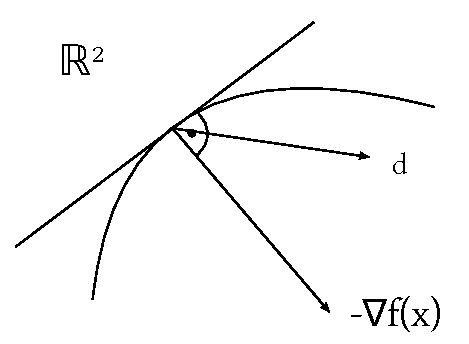
\includegraphics{img/25_descent.pdf}
			\caption{Geometrical interpretation of the descent}
		\end{center}
	\end{figure}
\end{Remark}
\begin{Remark}
	Colloquially the condition $(\nabla f(x))^t d < 0$ is used as definition of direction of descent.
\end{Remark}

We are going to use this condition in our algorithms.

\begin{Remark}[Observation]
	Let $f: \mathbb R^n \to \mathbb R$ be continuously differentiable and $x \in \mathbb R^n$. $x$ is not a stationary point of $f$.
	Let $B$ be a symmetric, positive definite $n\times n$ matrix. Then $d = -B \nabla f(x)$ is a direction of descent.

	\emph{Special case:} $d = -\nabla f(x)$ is a direction of descent. In particular, the direction of \emph{steepest descent}\index{Steepest descent}.
\end{Remark}

\begin{algorithm}[Generic descent method]\hfill{}
	\begin{enumerate}
		\item Choose $x^{(0)} \in \mathbb R^n$ and let $k \coloneqq 0$
		\item If $x^{(k)}$ suffices the chosen termination condition, then STOP.
		\item Determine a direction of descent $d^{(k)}$ of $f$ in $x^{(k)}$
		\item Determine a step size $t_k > 0$ with $f(x^{(k)} + t_k d^{(k)}) < f(x^{(k)})$
		\item Let $x^{(k+1)} \coloneqq x^{(k)} + t_k d^{(k)}$. Let $k \coloneqq k + 1$. Go to (1).
	\end{enumerate}
	Step size, direction of descent and termination condition are left to be discussed.
\end{algorithm}

For analysis of convergence, we consider the infinite sequence $\Set{x^{(k)}}, \Set{d^{(k)}}$ and $\Set{t_k}$ without satisfied termination condition. The central question for us is under which conditions of $d^{(k)}$ and $t_k$ we achieve convergence. With arbitrary chosen $d^{(k)}$ and $t_k$ we don't get a useful generic approach. We need to establish some conditions on $t_k$ and $d^{(k)}$.

\emph{Our goal:} Every cluster point of sequence $\Set{x^{(k)}}$ should be at least one stationary point of $f$.

\begin{Remark}[Find appropriate step size]
	Given $(x, d)$ with $x \in \mathbb R^n$ and $d \in \mathbb R^n$, find step size $t > 0$.

	Consider map $T$, that associates a subset $T(x, d)$ of $R^{++} = \SetDef{t \in R}{t > 0}$ to every $(x, d) \in \mathbb R^n \times \mathbb R^n$. We call $T$ a \emph{step size strategy}\index{Step size strategy} (or \emph{Step size rule}\index{Step size rule}).

	\index{Well-defined step size strategy}
	$T$ is called \emph{well-defined} if---under some particular conditions---the set $T(x, d)$ for every pair $(x, d) \in \mathbb R^n \times \mathbb R^n$ with $\left(\nabla f(x)\right)^t d < 0$ is non-empty.
\end{Remark}

\begin{definition}[Efficient step size strategy]
	Let $f: \mathbb R^n \to \mathbb R$ be continuously differentiable, $x \in \mathbb R^n$ and $d \in \mathbb R^n$ be a direction of descent of $f$ in $x$.
	A step size strategy $T$ is called \emph{efficient}\index{Efficient step size strategy}, if $\exists \theta > 0$ (of $x$ and $d$) such that
	\[ \forall t \in T(x, d): f(x + td) \leq f(x) - \theta \left(\frac{(\nabla f(x))^t d}{\Norm{d}}\right)^2 \]
\end{definition}

\begin{Remark}
	One motivating case for this definition is the special case of quadratic functions (compare with practicals).
\end{Remark}

In the next subchapter, we are going to discuss specific (efficient) step size strategies.

\begin{Definition}
	$t \in T(x, d)$ with efficient $T$ is called \emph{efficient step size}\index{Efficient step size}.
\end{Definition}

\begin{theorem}
	\label{theorem:5.3.2}
	Let $f: \mathbb R^n \to \mathbb R$ be continuously differentiable and let sequence $\Set{x^{(k)}}$ be generated by the generic descent method. If $\Set{x^{(k)}}$ is satisfies the two conditions (E1) and (E2), then every cluster point of $\Set{x^{(k)}}$ is a stationary point of $f$.

	Condition (E1) is called \enquote{angle condition}:
	\[ \exists c > 0 \forall k \in \mathbb N: \frac{-\left(\nabla f(x^{(k)})\right)^t d^{(k)}}{\Norm{\nabla f(x^{(k)})}\Norm{d^{(k)}}} \geq c \]
	Condition (E2) requires step sizes $t_k > 0$ are efficient for all $k \in \mathbb N$.
\end{theorem}

\begin{Remark}
	The direction of the steepest descent $d^{(k)} = -\nabla f(x^{(k)})$ satisfies the angle condition.
	More examples will be provided in the upcoming classes.
\end{Remark}

\begin{Remark}[About the angle condition E1]
	Let $\varphi_k$ be an angle between $d^{(k)}$ and $-\nabla f(x^{(k)})$. Then
	\[ \cos\varphi_k = -\frac{\left(\nabla f(x^{k})\right)^t d^{(k)}}{\Norm{\nabla f(x^k)}\Norm{d^{(k)}}} \]
	If this angle is smaller than $\frac\pi2$, then the direction of descent is $d^{(k)}$ by Lemma~\ref{lemma:5.3.1}.
	The condition (E1) states that the angle between $-\nabla f(x^{(k)})$ and $d^{(k)}$ is uniformly bounded (sufficiently far away from $\frac\pi2$).
\end{Remark}

\begin{proof}[Proof of Theorem~\ref{theorem:5.3.2}]
	For every efficient $t_k > 0$,
	\[ \exists \theta > 0: f(x^{(k+1)}) > f(x^{(k)} + t_k \cdot d^{(k)}) \leq f(x^{(k)}) - \theta \left(\frac{(\nabla f(x^{(k)}))^t d^{(k)}}{\Norm{d^{(k)}}}\right)^2 \forall k \in \mathbb N \]
	By E1, we get
	\[ (*): \quad f(x^{(k+1)}) \leq f(x^{(k)}) - \kappa \cdot \Norm{\nabla f(x^{(k)})}^2 \text{ with } \kappa \coloneqq \theta c^2 \]
	Now let $x^*$ be a cluster point of $\Set{x^{(k)}}$.

	The sequence $\Set{f(x^{(k)})}$ is monotonically decreasing and converges on a subsequence towards $f(x^*)$.
	Thus $\Set{f(x^{(k)})}$ converges towards $f(x^*)$.
	\[ \implies f(x^{(k+1)}) - f(x^{(k)}) \to 0 \qquad \xRightarrow{(*)} \Norm{\nabla f(x^{(k)})} \to 0 \]
	Thus every accumulation point of $\Set{x^{(k)}}$ is a stationary point of $f$.
\end{proof}

A second convergence result requires a weakening of the angle condition.
(E1) forbids sequence $\frac\pi2$ to approach $\Set{\varphi_k}$. In this case, we discard this requirement, but it must not happen too fast.

\begin{theorem}
	\label{theorem:5.3.3}
	Let $f: \mathbb R^n \to \mathbb R$ be continuously differentiable. The level set $\mathcal L(x^{(0)}) = \SetDef{x \in \mathbb R^n}{f(x) \leq f(x^{(k)})}$ is convex and $f$ is uniformly convex on $\mathcal L(x^{(0)})$.
	Let $\Set{x^{(k)}}$ be the iteration sequence generated by the descent method satisfying
	\begin{description}
		\item[$\overline{E1}$ (\enquote{Zouten dijk condition})] $\sum_{k=0}^\infty \delta_k = \infty$ with
			\[ \delta_k = \left(\frac{\left(\nabla f(x^{(k)})\right)^t d^{(k)}}{\Norm{\nabla f(x^{(k)})}}\right) \]
		\item[$\overline{E2}$] as before
	\end{description}
	In this case, $\Set{x^{(k)}}$ converges towards the uniquely determined global minimum of $f$
\end{theorem}

\printindex
\end{document}